% HealthStack project report.
% Compile from this folder (docs/report/):  pdflatex HealthStack_Report.tex  (run twice)
% Images: ../diagrams/HealthStack_ER_updated.jpg and screenshots/*.png
\documentclass[11pt,a4paper]{article}

\usepackage[T1]{fontenc}
\usepackage[utf8]{inputenc}
\usepackage{lmodern}
\usepackage[margin=2.2cm]{geometry}
\usepackage{amsmath,amssymb}
\usepackage{graphicx}
\usepackage{float}
\usepackage{caption}
\usepackage{subcaption}
\usepackage{booktabs}
\usepackage{tabularx}
\usepackage{longtable}
\usepackage{array}
\usepackage{enumitem}
\usepackage{xcolor}
\usepackage{listings}
\usepackage{tikz}
\usetikzlibrary{positioning,arrows.meta}
\usepackage{fancyhdr}
\usepackage[hidelinks]{hyperref}

% ---------------------------------------------------------------- edit these
\newcommand{\CourseName}{\TBD{Course name and code}}
\newcommand{\Instructor}{\TBD{Instructor}}
\newcommand{\Institute}{\TBD{Institute}}
\newcommand{\RepoURL}{https://github.com/shubhamsharma024680-lab/health-stack}
% ---------------------------------------------------------------------------

\newcommand{\TBD}[1]{\textcolor{red}{[#1]}}
\newcommand{\code}[1]{\texttt{#1}}
\newcommand{\fk}{$\rightarrow$\,}
\newcommand{\yes}{$\checkmark$}
\newcommand{\no}{$\times$}
\newcolumntype{L}{>{\raggedright\arraybackslash}X}
\newcolumntype{P}[1]{>{\raggedright\arraybackslash}p{#1}}

\setlist{itemsep=2pt,topsep=4pt}
\setlength{\parskip}{5pt}
\setlength{\parindent}{0pt}
\renewcommand{\arraystretch}{1.22}
\captionsetup{font=small,labelfont=bf}

\definecolor{codebg}{RGB}{246,247,249}
\definecolor{codekw}{RGB}{0,92,158}
\definecolor{codecm}{RGB}{110,120,130}
\definecolor{codest}{RGB}{150,60,20}
\lstset{
  basicstyle=\ttfamily\footnotesize,
  backgroundcolor=\color{codebg},
  keywordstyle=\color{codekw}\bfseries,
  commentstyle=\color{codecm}\itshape,
  stringstyle=\color{codest},
  breaklines=true,
  columns=fullflexible,
  keepspaces=true,
  frame=single,
  rulecolor=\color{codebg},
  xleftmargin=4pt,
  xrightmargin=4pt,
  aboveskip=6pt,
  belowskip=6pt
}
\lstdefinestyle{sql}{language=SQL, morekeywords={START,TRANSACTION,COMMIT,ROLLBACK,FOR,TRUE,NULL,JOIN,ON,DESC,TRIGGER,BEFORE,EACH,ROW,BEGIN,END,IF,THEN,SIGNAL,SQLSTATE,MESSAGE_TEXT,EXISTS,COALESCE,SUM,NEW,OLD,DELIMITER,GENERATED,STORED,UNIQUE,CHECK,REFERENCES,CASCADE,RESTRICT,AUTO_INCREMENT}}
\lstdefinestyle{bash}{language=bash, morecomment=[l]{--}}
\lstdefinestyle{py}{language=Python}

\pagestyle{fancy}
\fancyhf{}
\fancyhead[L]{\small HealthStack}
\fancyhead[R]{\small Project report}
\fancyfoot[C]{\small\thepage}
\renewcommand{\headrulewidth}{0.4pt}

\begin{document}

% ============================================================== title page
\begin{titlepage}
\centering
\vspace*{2.5cm}
{\Huge\bfseries HealthStack\par}
\vspace{0.4cm}
{\Large A hospital management system on MySQL\par}
\vspace{1.5cm}
{\large Project report\par}
\vspace{0.3cm}
{\large \CourseName\par}
\vspace{0.2cm}
{\large Instructor: \Instructor\par}
\vspace{2cm}
\begin{tabular}{ll}
\toprule
\textbf{Name} & \textbf{Roll no.} \\
\midrule
Darshik Ladhe   & \TBD{roll no.} \\
Deepak Chahar   & \TBD{roll no.} \\
Shubham Sharma  & \TBD{roll no.} \\
Kedar Hadnurkar & \TBD{roll no.} \\
\bottomrule
\end{tabular}
\vfill
{\large \Institute\par}
\vspace{0.2cm}
{\large November 2026\par}
\end{titlepage}

\tableofcontents
\newpage

% ============================================================== 1
\section{What we are building}

HealthStack is a hospital management system built around a MySQL database. It covers the part of a hospital's day that a patient actually sees: finding a doctor, booking a time slot, the consultation, the prescription and the bill. The web interface is branded \emph{Careflow}.

There are three kinds of users, and each gets their own screens:

\begin{itemize}
  \item \textbf{Patients} register and log in, browse departments and doctors, see a doctor's free slots, and book, cancel or reschedule appointments. They can see every past visit with its prescription and bill, and a dashboard of upcoming visits, running prescriptions and unpaid bills.
  \item \textbf{Doctors} see today's queue. Opening an appointment shows the patient's details and their full visit history across all doctors. Completing a visit records the prescription, and the system creates the bill automatically.
  \item \textbf{Pharmacists} see every unpaid bill with the medicines to dispense, and record payments.
\end{itemize}

The database is the core of the project. It does more than store rows: constraints and triggers enforce the hospital's rules, such as no double-booking, no prescription for a cancelled visit, and no change to a bill once it is issued. These rules hold no matter which program writes the data. Every multi-step action, like completing a visit, runs as one transaction, so it either completes fully or leaves nothing behind.

\begin{center}
\small
\begin{tabularx}{\textwidth}{l L L}
\toprule
\textbf{Layer} & \textbf{Technology} & \textbf{Folder} \\
\midrule
Database & MySQL 8.0.16+ (16 tables, 25 triggers, 1 stored procedure) & \code{backend/schema}, \code{backend/seed}, \code{backend/triggers} \\
Backend  & Python 3, FastAPI, \code{mysql-connector-python} (21 endpoints) & \code{backend/} \\
Frontend & React 19, Vite, Tailwind CSS, React Router & \code{frontend/} \\
\bottomrule
\end{tabularx}
\end{center}

\textbf{Scope.} Hospital staff structure (employees, doctors, nurses, ward boys, receptionists, pharmacists, wards, departments) is fully modelled in the database. The application workflows cover outpatient care: appointments, prescriptions and billing. Ward admissions and technicians appear in the ER diagram as planned extensions.

% ============================================================== 2
\section{Team}

\begin{center}
\small
\begin{tabularx}{\textwidth}{P{3.3cm} P{2.4cm} L}
\toprule
\textbf{Member} & \textbf{Roll no.} & \textbf{Main contributions} \\
\midrule
Darshik Ladhe   & \TBD{roll no.} & FastAPI backend and its APIs (authentication, appointments, billing), triggers, seed data \\
Deepak Chahar   & \TBD{roll no.} & Schema design and fixes, ER diagram, frontend and its tests, documentation \\
Shubham Sharma  & \TBD{roll no.} & Transactions, grouping the triggers and aligning them with the schema \\
Kedar Hadnurkar & \TBD{roll no.} & Repository configuration \\
\bottomrule
\end{tabularx}
\end{center}

% ============================================================== 3
\section{Getting started}

\subsection{Prerequisites}

\begin{itemize}
  \item Git
  \item MySQL 8.0.16 or newer. Older versions silently ignore \code{CHECK} constraints. MariaDB also works; the schema was tested on MariaDB 13.
  \item Python 3.10 or newer
  \item Node.js 20.19 or newer (needed by Vite)
\end{itemize}

\subsection{Clone the repository}

\begin{lstlisting}[style=bash]
git clone https://github.com/shubhamsharma024680-lab/health-stack.git
cd health-stack
\end{lstlisting}

\subsection{Create the database}

Run both scripts from the project root, inside the MySQL client. \code{table.sql} drops and recreates every table and installs all triggers; \code{seed.sql} loads the demo data. Running both again resets the demo.

\begin{lstlisting}[style=bash]
mysql -u root -p
mysql> SOURCE backend/schema/table.sql;
mysql> SOURCE backend/seed/seed.sql;
\end{lstlisting}

The last statement prints \code{Demo ready} and the number of accounts per role (10 patients, 4 doctors, 2 pharmacists).

\subsection{Start the backend}

\begin{lstlisting}[style=bash]
cd backend
python -m venv .venv
source .venv/bin/activate          # Windows: .venv\Scripts\activate
pip install -r requirements.txt
cp .env.example .env               # then set My_SQL_USER and My_SQL_PASSWORD
python server.py                   # serves http://127.0.0.1:8000
\end{lstlisting}

Open \url{http://127.0.0.1:8000/health/db}; it should return \code{\{"database": "connected"\}}. Interactive API documentation is at \url{http://127.0.0.1:8000/docs}.

\subsection{Start the frontend}

In a second terminal:

\begin{lstlisting}[style=bash]
cd frontend
cp .env.example .env               # VITE_API_URL=http://127.0.0.1:8000
npm install
npm run dev                        # serves http://localhost:5173
\end{lstlisting}

\subsection{Log in}

Open \url{http://localhost:5173}, pick a role and sign in. Every demo account uses the password \code{demo123}.

\begin{center}
\small
\begin{tabular}{lll}
\toprule
\textbf{Role} & \textbf{Email} & \textbf{Who} \\
\midrule
Patient    & \code{patient@demo.com}    & Aarav Mehta \\
Doctor     & \code{doctor@demo.com}     & Dr.\ Meera Iyer (General Medicine) \\
Pharmacist & \code{pharmacist@demo.com} & Riya Shah \\
\bottomrule
\end{tabular}
\end{center}

% ============================================================== 4
\section{ER diagram}

\begin{figure}[H]
\centering
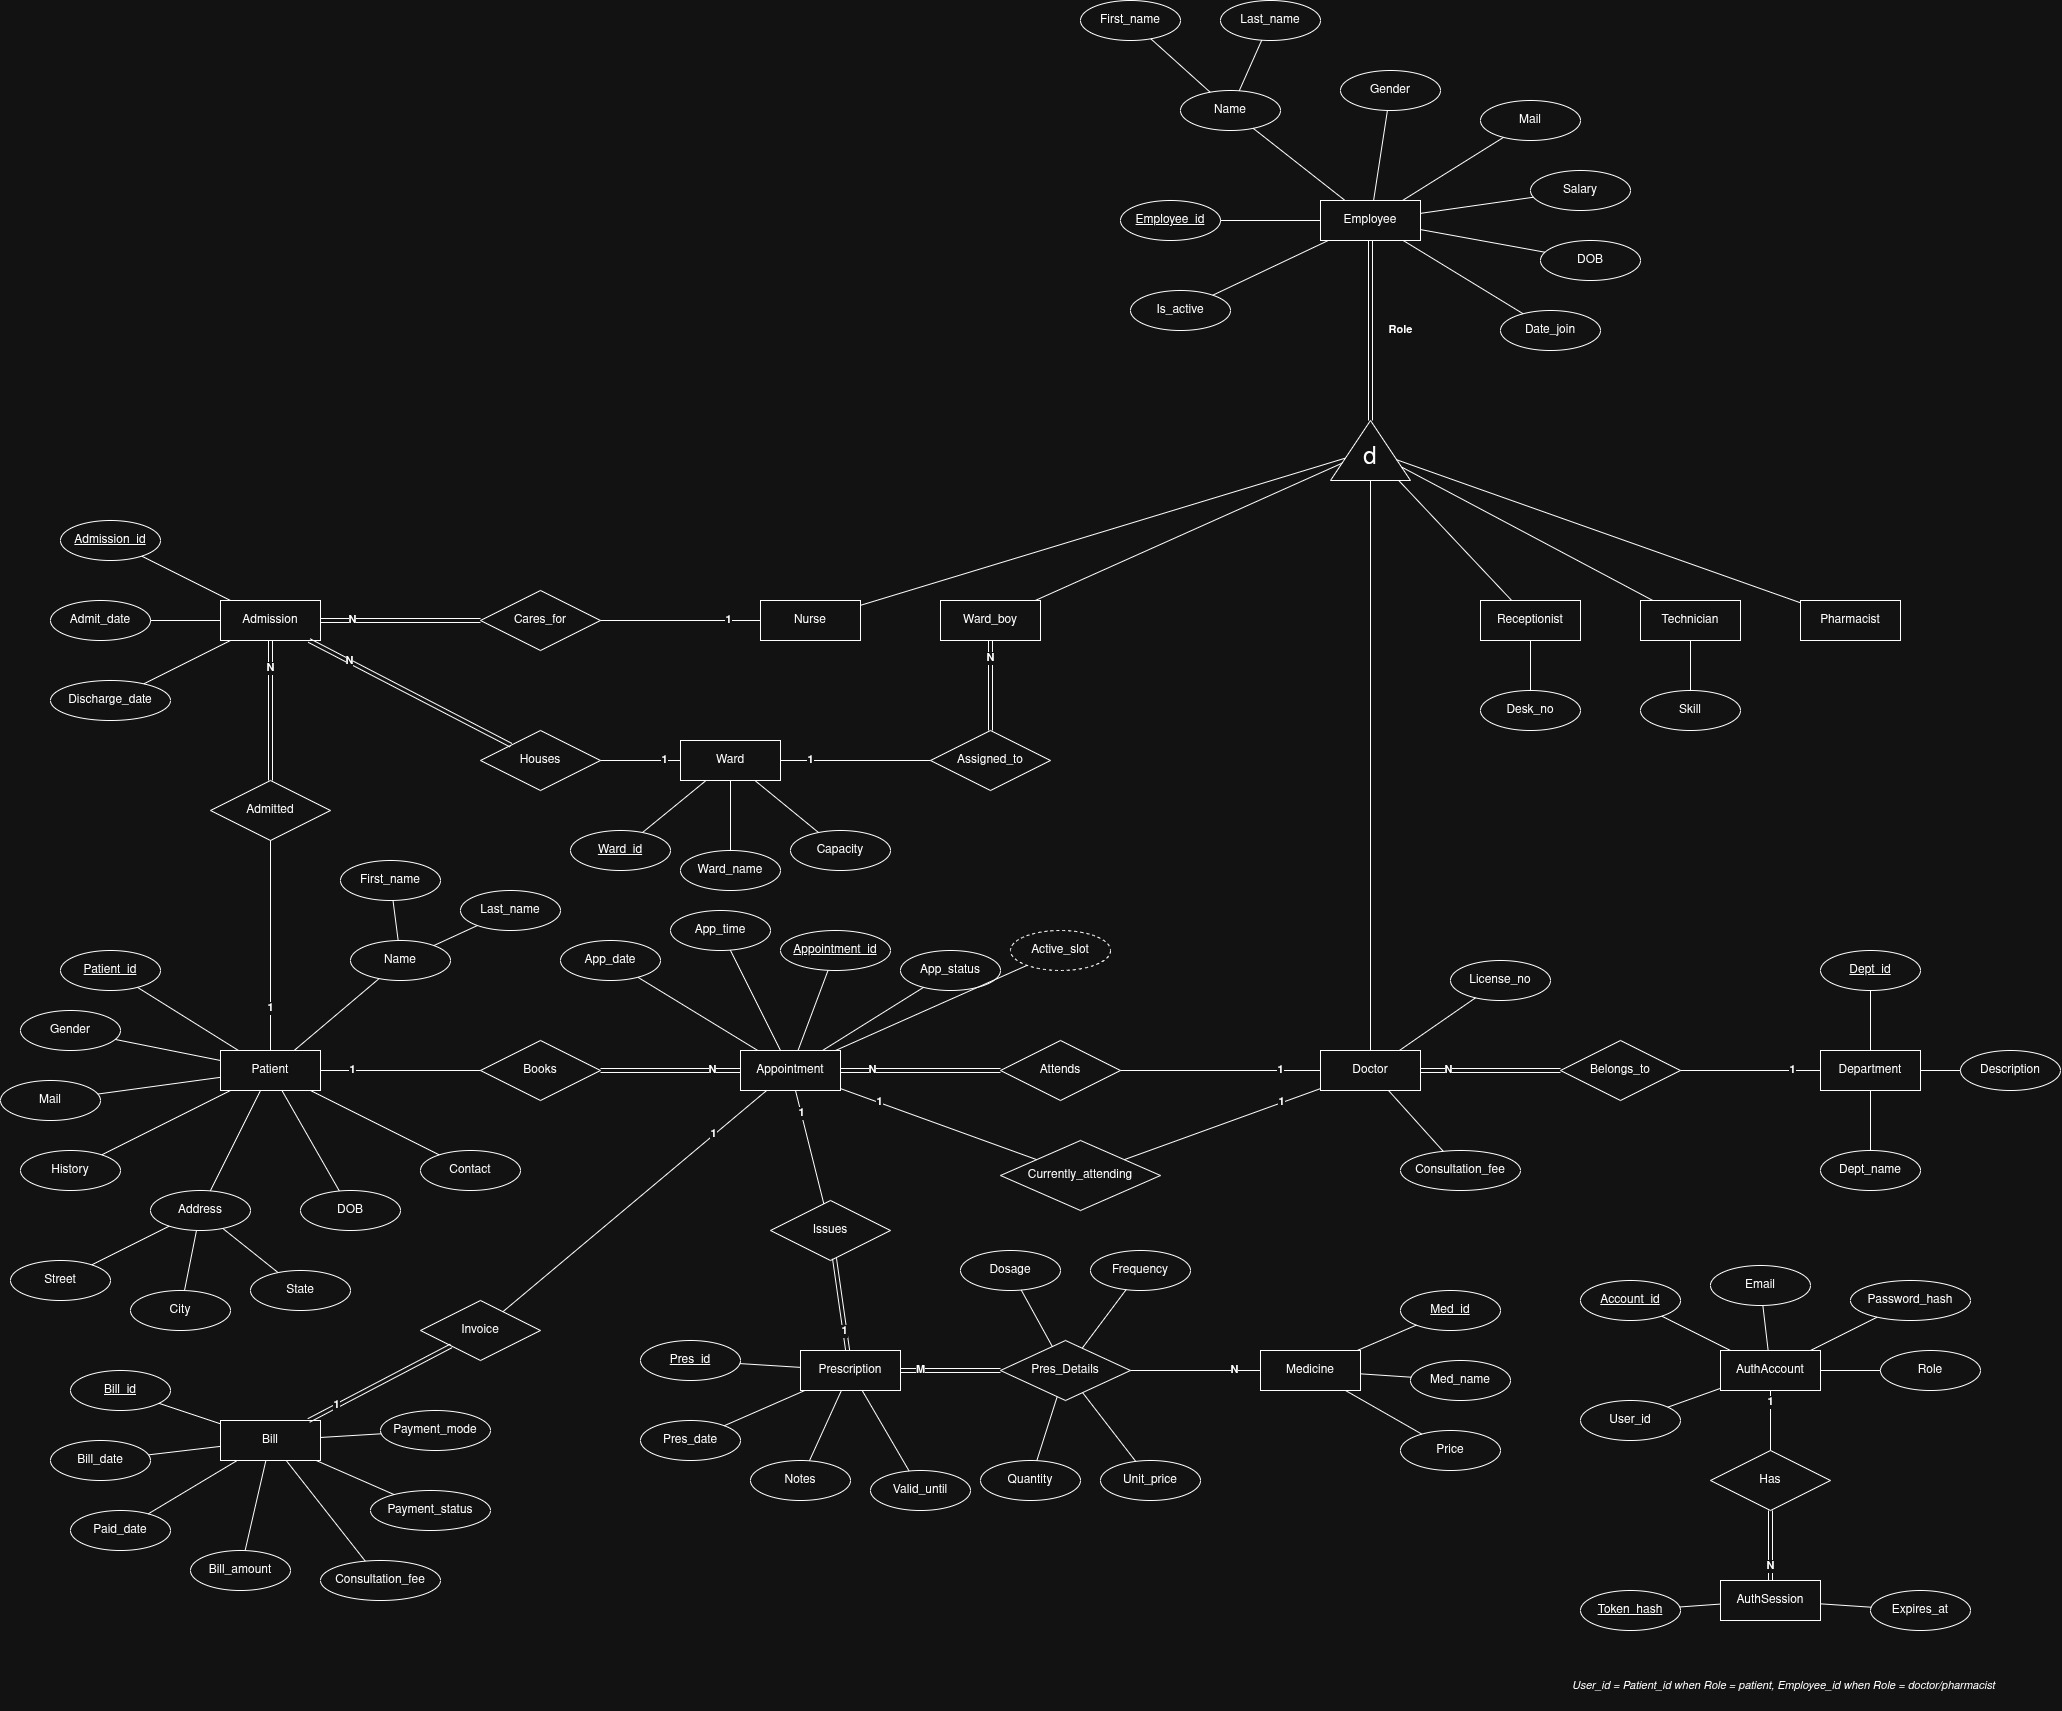
\includegraphics[width=\textwidth]{../diagrams/HealthStack_ER_updated.jpg}
\caption{HealthStack ER diagram}
\end{figure}

\subsection{Entities and specialisation}

\begin{itemize}
  \item \textbf{Employee} is the superclass of all staff. It is specialised into Doctor, Nurse, Ward\_boy, Receptionist, Technician and Pharmacist. The specialisation is \textbf{disjoint} (the \code{d} in the triangle: one employee is in at most one subclass), \textbf{total} (double line: every employee is in some subclass) and \textbf{attribute-defined} by \code{Role}.
  \item \code{Name} (\code{First\_name}, \code{Last\_name}) and \code{Address} (\code{Street}, \code{City}, \code{State}) are \textbf{composite} attributes.
  \item \code{Active\_slot} on Appointment is a \textbf{derived} attribute (dashed ellipse).
  \item \textbf{AuthAccount} and \textbf{AuthSession} hold logins and signed-in sessions. \code{User\_id} is a \code{Patient\_id} when \code{Role} = patient and an \code{Employee\_id} otherwise.
\end{itemize}

\subsection{Relationships}

\begin{center}
\small
\begin{tabularx}{\textwidth}{l l c L}
\toprule
\textbf{Relationship} & \textbf{Between} & \textbf{Cardinality} & \textbf{Notes} \\
\midrule
Books               & Patient -- Appointment      & 1 : N & Every appointment has a patient (total) \\
Attends             & Doctor -- Appointment       & 1 : N & Every appointment has a doctor (total) \\
Currently\_attending & Doctor -- Appointment      & 1 : 1 & The visit a doctor is in right now (partial) \\
Belongs\_to         & Department -- Doctor        & 1 : N & Every doctor is in a department (total) \\
Issues              & Appointment -- Prescription & 1 : 1 & At most one prescription per visit \\
Invoice             & Appointment -- Bill         & 1 : 1 & At most one bill per visit \\
Pres\_Details       & Prescription -- Medicine    & M : N & Attributes: Dosage, Quantity, Frequency, Unit\_price \\
Assigned\_to        & Ward -- Ward\_boy           & 1 : N & Every ward boy has a ward (total) \\
Has                 & AuthAccount -- AuthSession  & 1 : N & One account, many sessions \\
Admitted, Houses, Cares\_for & Patient, Ward, Nurse -- Admission & 1 : N & Planned; not yet tables \\
\bottomrule
\end{tabularx}
\end{center}

\subsection{Mapping the ER model to tables}

\begin{itemize}
  \item Composite attributes are split into one column per part.
  \item Each subclass becomes its own table whose primary key is also a foreign key to \code{Employee} (\code{ON DELETE CASCADE}). Triggers enforce that the subclass matches \code{Employee.Role}.
  \item 1:N relationships become a foreign key on the N side, \code{NOT NULL} where participation is total.
  \item 1:1 relationships (Issues, Invoice) become a \code{UNIQUE NOT NULL} foreign key.
  \item The M:N relationship Pres\_Details becomes a junction table with the composite key (\code{Pres\_id}, \code{Med\_id}) and its four attributes.
  \item The derived \code{Active\_slot} becomes a \code{STORED} generated column (section~\ref{sec:schemas}).
\end{itemize}

% ============================================================== 5
\section{Normal forms}

\subsection{Definitions}

Let $R$ be a relation and $X$, $Y$ sets of its attributes. A \textbf{functional dependency} (FD) $X \rightarrow Y$ means any two rows that agree on $X$ also agree on $Y$; it is \emph{trivial} if $Y \subseteq X$. A \textbf{candidate key} is a minimal set of attributes that determines all of $R$. An attribute is \textbf{prime} if it belongs to some candidate key.

\begin{itemize}
  \item \textbf{1NF}: every attribute holds a single atomic value, and the relation has a key (no duplicate rows).
  \item \textbf{2NF}: 1NF, and no non-prime attribute depends on a proper subset of a candidate key (no partial dependency). A relation whose candidate keys are all single attributes is automatically in 2NF.
  \item \textbf{3NF}: for every non-trivial FD $X \rightarrow A$, either $X$ is a superkey or $A$ is prime. This rules out transitive dependencies $\text{key} \rightarrow X \rightarrow A$.
  \item \textbf{BCNF}: for every non-trivial FD $X \rightarrow A$, $X$ is a superkey.
\end{itemize}

\textbf{Method.} For each table we list the FDs that the schema enforces (primary keys, \code{UNIQUE NOT NULL} columns, generated columns, values forced by triggers). For dependencies one might expect, we show why they do not hold, using the seed data or the application's rules. Checks that compare two values in the same row, such as \code{Date\_join > DOB}, are constraints, not FDs, and do not affect the normal form.

\subsection{Summary}

\begin{center}
\small
\begin{tabularx}{\textwidth}{l L c c c c}
\toprule
\textbf{Table} & \textbf{Candidate keys} & \textbf{1NF} & \textbf{2NF} & \textbf{3NF} & \textbf{BCNF} \\
\midrule
Department   & \{Dept\_id\}, \{Dept\_name\}                 & \yes & \yes & \yes & \yes \\
Employee     & \{Employee\_id\}, \{Mail\}                   & \yes & \yes & \yes & \yes \\
Doctor       & \{Employee\_id\}, \{License\_no\}            & \yes & \yes & \yes & \yes \\
Nurse        & \{Employee\_id\}                             & \yes & \yes & \yes & \yes \\
Ward         & \{Ward\_id\}, \{Ward\_name\}                 & \yes & \yes & \yes & \yes \\
Ward\_boy    & \{Employee\_id\}                             & \yes & \yes & \yes & \yes \\
Receptionist & \{Employee\_id\}                             & \yes & \yes & \yes & \yes \\
Pharmacist   & \{Employee\_id\}                             & \yes & \yes & \yes & \yes \\
Patient      & \{Patient\_id\}                              & \yes & \yes & \yes & \yes \\
Appointment  & \{Appointment\_id\}                          & \yes & \yes & \no  & \no  \\
Prescription & \{Pres\_id\}, \{Appointment\_id\}            & \yes & \yes & \yes & \yes \\
Medicine     & \{Med\_id\}                                  & \yes & \yes & \yes & \yes \\
Pres\_Details & \{Pres\_id, Med\_id\}                       & \yes & \yes & \yes & \yes \\
Bill         & \{Bill\_id\}, \{Appointment\_id\}            & \yes & \yes & \no  & \no  \\
AuthAccount  & \{Account\_id\}, \{Email\}, \{Role, User\_id\} & \yes & \yes & \yes & \yes \\
AuthSession  & \{Token\_hash\}                              & \yes & \yes & \yes & \yes \\
\bottomrule
\end{tabularx}
\end{center}

\textbf{14 of the 16 tables are in BCNF.} Appointment and Bill reach 2NF; both cases are explained below, with the fix or the reason it is acceptable.

\subsection{Derivations}

\subsubsection*{Department and Ward}
$\text{Department}(\underline{\text{Dept\_id}}, \text{Dept\_name}, \text{Description})$, $\text{Ward}(\underline{\text{Ward\_id}}, \text{Ward\_name}, \text{Capacity})$.

\textbf{FDs:} $\text{Dept\_id} \rightarrow \text{Dept\_name}, \text{Description}$ and $\text{Dept\_name} \rightarrow \text{Dept\_id}, \text{Description}$ (\code{Dept\_name} is \code{UNIQUE NOT NULL}). The same holds for \code{Ward\_id} and \code{Ward\_name}. \code{Description} and \code{Capacity} determine nothing: two wards can have the same capacity.

\textbf{Result:} every determinant is a candidate key, so both tables are in \textbf{BCNF}.

\subsubsection*{Employee}
$\text{Employee}(\underline{\text{Employee\_id}}, \text{First\_name}, \text{Last\_name}, \text{Gender}, \text{DOB}, \text{Date\_join}, \text{Mail}, \text{Salary}, \text{Role}, \text{Is\_active})$.

\textbf{FDs:} $\text{Employee\_id} \rightarrow \text{all}$; $\text{Mail} \rightarrow \text{all}$ (\code{UNIQUE NOT NULL}).
\textbf{Not FDs:} $\text{Role} \nrightarrow \text{Salary}$ (doctors 101 and 102 earn 120000 and 140000); a name is not unique.

\textbf{Result:} both determinants are keys, so \textbf{BCNF}.

\subsubsection*{Doctor}
$\text{Doctor}(\underline{\text{Employee\_id}}, \text{License\_no}, \text{Current\_appointment\_id}, \text{Dept\_id}, \text{Consultation\_fee})$.

\textbf{FDs:} $\text{Employee\_id} \rightarrow \text{all}$; $\text{License\_no} \rightarrow \text{all}$.
\textbf{Not FDs:} $\text{Dept\_id} \nrightarrow \text{Consultation\_fee}$: the fee is stored per doctor, and departments have several doctors. \code{Current\_appointment\_id} is nullable and shared by many doctors as \code{NULL}, so it determines nothing.

\textbf{Result:} \textbf{BCNF}.

\subsubsection*{Nurse, Pharmacist, Ward\_boy and Receptionist}
Nurse and Pharmacist have the single attribute \code{Employee\_id}, so they have no non-trivial FDs and are in BCNF. Ward\_boy(\underline{Employee\_id}, Ward\_id) has only $\text{Employee\_id} \rightarrow \text{Ward\_id}$; a ward has several ward boys, so $\text{Ward\_id} \nrightarrow \text{Employee\_id}$. Receptionist(\underline{Employee\_id}, Desk\_no) has only $\text{Employee\_id} \rightarrow \text{Desk\_no}$; desks can be shared.

\textbf{Result:} all four are in \textbf{BCNF}.

\subsubsection*{Patient}
$\text{Patient}(\underline{\text{Patient\_id}}, \text{First\_name}, \text{Last\_name}, \text{Gender}, \text{DOB}, \text{Mail}, \text{Contact}, \text{Street}, \text{City}, \text{State}, \text{History})$.

\textbf{FDs:} $\text{Patient\_id} \rightarrow \text{all}$.
\textbf{Not FDs:} \code{Mail} and \code{Contact} are not keys (\code{Mail} is nullable, and family members may share a phone or email). $\text{City} \nrightarrow \text{State}$, because city names repeat across states (Aurangabad is in Maharashtra and in Bihar). The composite ER attributes are already split into atomic columns, so the table is in 1NF.

\textbf{Result:} \textbf{BCNF}.

\subsubsection*{Appointment (2NF)}
$\text{Appointment}(\underline{\text{Appointment\_id}}, \text{Patient\_id}, \text{Doctor\_id}, \text{App\_date}, \text{App\_time}, \text{App\_status}, \text{Active\_slot})$.

\textbf{FDs:} $\text{Appointment\_id} \rightarrow \text{all}$, and $\text{App\_status} \rightarrow \text{Active\_slot}$, because \code{Active\_slot} is the generated column \code{IF(App\_status = 'Cancelled', NULL, 1)}.
\textbf{Not keys:} (\code{Doctor\_id}, \code{App\_date}, \code{App\_time}) is not a key, since a cancelled appointment and a new booking can share a slot. The \code{UNIQUE} index that includes \code{Active\_slot} is not a candidate key either, because \code{Active\_slot} is \code{NULL} for cancelled rows.

\begin{center}
\small
\begin{tabularx}{0.92\textwidth}{l c L}
\toprule
\textbf{Form} & \textbf{Holds?} & \textbf{Reason} \\
\midrule
1NF  & \yes & Atomic values, primary key \\
2NF  & \yes & The only candidate key is a single attribute \\
3NF  & \no  & $\text{App\_status} \rightarrow \text{Active\_slot}$: App\_status is not a superkey and Active\_slot is not prime. This is the transitive chain $\text{Appointment\_id} \rightarrow \text{App\_status} \rightarrow \text{Active\_slot}$ \\
BCNF & \no  & Fails for the same FD \\
\bottomrule
\end{tabularx}
\end{center}

\textbf{Why this is acceptable.} The column exists only to stop double-booking: \code{UNIQUE (Doctor\_id, App\_date, App\_time, Active\_slot)} must ignore cancelled appointments, and MySQL has no filtered unique index. Moving \code{Active\_slot} to another table (the 3NF decomposition) would make that constraint span two tables, which SQL cannot enforce. The anomaly 3NF guards against cannot happen here: MySQL computes the column, and nobody can write it. Without \code{Active\_slot} the table is in BCNF.

\subsubsection*{Prescription and Medicine}
Prescription(\underline{Pres\_id}, Appointment\_id, Pres\_date, Notes, Valid\_until) has $\text{Pres\_id} \rightarrow \text{all}$ and $\text{Appointment\_id} \rightarrow \text{all}$ (\code{UNIQUE NOT NULL}: one prescription per visit). $\text{Pres\_date} \nrightarrow \text{Valid\_until}$, because the doctor chooses the validity per prescription. Medicine(\underline{Med\_id}, Med\_name, Price) has only $\text{Med\_id} \rightarrow \text{all}$; \code{Med\_name} is not declared unique.

\textbf{Result:} both are in \textbf{BCNF}.

\subsubsection*{Pres\_Details}
$\text{Pres\_Details}(\underline{\text{Pres\_id}, \text{Med\_id}}, \text{Dosage}, \text{Quantity}, \text{Frequency}, \text{Unit\_price})$.

\textbf{FDs:} $(\text{Pres\_id}, \text{Med\_id}) \rightarrow \text{Dosage}, \text{Quantity}, \text{Frequency}, \text{Unit\_price}$.

\textbf{2NF check (partial dependencies):}
\begin{itemize}
  \item $\text{Pres\_id} \nrightarrow \text{Quantity}$: prescription 1 lists 10 of medicine 1 and 2 of medicine 2.
  \item $\text{Med\_id} \nrightarrow \text{Quantity}$: medicine 1 is 10 tablets in prescription 1 and 6 in prescription 6.
  \item $\text{Med\_id} \nrightarrow \text{Unit\_price}$: trigger \code{trg\_pres\_details\_bi} copies \code{Medicine.Price} when the line is inserted and \code{trg\_pres\_details\_bu} keeps it afterwards. \code{Unit\_price} is the price \emph{at the time of prescribing}, so after a price change the same medicine has different unit prices in old and new prescriptions.
\end{itemize}

\textbf{Result:} the only determinant is the key, so \textbf{BCNF}. If \code{Unit\_price} simply mirrored today's price, $\text{Med\_id} \rightarrow \text{Unit\_price}$ would be a partial dependency and the table would drop to 1NF; storing a snapshot is what keeps it normalised.

\subsubsection*{Bill (2NF)}
$\text{Bill}(\underline{\text{Bill\_id}}, \text{Appointment\_id}, \text{Consultation\_fee}, \text{Bill\_amount}, \text{Bill\_date}, \text{Paid\_date}, \text{Payment\_status}, \text{Payment\_mode})$.

\textbf{FDs:} $\text{Bill\_id} \rightarrow \text{all}$; $\text{Appointment\_id} \rightarrow \text{all}$ (one bill per visit); and $\emptyset \rightarrow \text{Consultation\_fee}$, because trigger \code{trg\_bill\_bi} sets the fee to 200 on every insert and \code{trg\_bill\_bu} never lets it change. A constant column is determined by every set of attributes, for example $\text{Bill\_date} \rightarrow \text{Consultation\_fee}$.
\textbf{Not FDs:} \code{Bill\_amount} is computed from the visit's prescription, which within Bill is just $\text{Appointment\_id} \rightarrow \text{Bill\_amount}$, already implied by the key. \code{Paid\_date}, \code{Payment\_status} and \code{Payment\_mode} are not linked by any FD.

\begin{center}
\small
\begin{tabularx}{0.92\textwidth}{l c L}
\toprule
\textbf{Form} & \textbf{Holds?} & \textbf{Reason} \\
\midrule
1NF  & \yes & Atomic values, primary key \\
2NF  & \yes & All candidate keys are single attributes \\
3NF  & \no  & $\text{Bill\_date} \rightarrow \text{Consultation\_fee}$: the determinant is not a superkey and the fee is not prime \\
BCNF & \no  & Fails for the same FD \\
\bottomrule
\end{tabularx}
\end{center}

\textbf{Fix.} Make \code{trg\_bill\_bi} copy the doctor's own \code{Doctor.Consultation\_fee} instead of the constant 200. The column then records the fee at billing time, the constant FD disappears, and Bill is in BCNF. This also fixes the billing logic, which today ignores per-doctor fees.

\subsubsection*{AuthAccount and AuthSession}
AuthAccount(\underline{Account\_id}, Email, Password\_hash, Role, User\_id) has three candidate keys: \{Account\_id\}, \{Email\} and \{Role, User\_id\} (\code{UNIQUE}, both \code{NOT NULL}). For 2NF, neither part of the composite key determines anything alone: many accounts share a role, and a \code{User\_id} number can be both a patient and an employee. AuthSession(\underline{Token\_hash}, Account\_id, Expires\_at) has only $\text{Token\_hash} \rightarrow \text{all}$; an account can have several sessions.

\textbf{Result:} both are in \textbf{BCNF}.

% ============================================================== 6
\section{Table schemas}
\label{sec:schemas}

All tables are created by \code{backend/schema/table.sql}. PK = primary key, FK = foreign key, NN = \code{NOT NULL}, AI = \code{AUTO\_INCREMENT}.

\small
\begin{longtable}{P{3.4cm} P{2.8cm} P{9.0cm}}
\toprule
\textbf{Column} & \textbf{Type} & \textbf{Constraints} \\
\midrule
\endfirsthead
\toprule
\textbf{Column} & \textbf{Type} & \textbf{Constraints} \\
\midrule
\endhead
\bottomrule
\endfoot

\multicolumn{3}{l}{\textbf{Department}} \\
Dept\_id & INT & PK \\
Dept\_name & VARCHAR(100) & UNIQUE, NN \\
Description & TEXT & \\
\midrule
\multicolumn{3}{l}{\textbf{Employee}} \\
Employee\_id & INT & PK \\
First\_name, Last\_name & VARCHAR(50) & NN \\
Gender & VARCHAR(10) & NN; CHECK in (Male, Female, Other) \\
DOB & DATE & NN \\
Date\_join & DATE & NN; CHECK (Date\_join > DOB) \\
Mail & VARCHAR(100) & UNIQUE, NN \\
Salary & DECIMAL(10,2) & NN; CHECK (Salary >= 0) \\
Role & VARCHAR(20) & NN; CHECK in (Doctor, Nurse, Ward\_boy, Receptionist, Technician, Pharmacist) \\
Is\_active & BOOLEAN & NN, DEFAULT TRUE \\
\midrule
\multicolumn{3}{l}{\textbf{Doctor}} \\
Employee\_id & INT & PK; FK \fk Employee ON DELETE CASCADE \\
License\_no & VARCHAR(50) & UNIQUE, NN \\
Current\_appointment\_id & INT & NULL allowed \\
Dept\_id & INT & NN; FK \fk Department ON DELETE RESTRICT \\
Consultation\_fee & DECIMAL(10,2) & NN, DEFAULT 200; CHECK (>= 0) \\
\midrule
\multicolumn{3}{l}{\textbf{Nurse}, \textbf{Pharmacist}} \\
Employee\_id & INT & PK; FK \fk Employee ON DELETE CASCADE \\
\midrule
\multicolumn{3}{l}{\textbf{Ward}} \\
Ward\_id & INT & PK \\
Ward\_name & VARCHAR(50) & UNIQUE, NN \\
Capacity & INT & NN; CHECK (Capacity > 0) \\
\midrule
\multicolumn{3}{l}{\textbf{Ward\_boy}} \\
Employee\_id & INT & PK; FK \fk Employee ON DELETE CASCADE \\
Ward\_id & INT & NN; FK \fk Ward ON DELETE RESTRICT \\
\midrule
\multicolumn{3}{l}{\textbf{Receptionist}} \\
Employee\_id & INT & PK; FK \fk Employee ON DELETE CASCADE \\
Desk\_no & VARCHAR(20) & NN \\
\midrule
\multicolumn{3}{l}{\textbf{Patient}} \\
Patient\_id & INT & PK, AI \\
First\_name, Last\_name & VARCHAR(50) & NN \\
Gender & VARCHAR(10) & NN; CHECK in (Male, Female, Other) \\
DOB & DATE & NN \\
Mail & VARCHAR(100) & \\
Contact & VARCHAR(20) & NN \\
Street & VARCHAR(100) & \\
City, State & VARCHAR(50) & \\
History & TEXT & \\
\midrule
\multicolumn{3}{l}{\textbf{Appointment}} \\
Appointment\_id & INT & PK, AI \\
Patient\_id & INT & NN; FK \fk Patient ON DELETE RESTRICT \\
Doctor\_id & INT & NN; FK \fk Doctor ON DELETE RESTRICT \\
App\_date & DATE & NN \\
App\_time & TIME & NN \\
App\_status & VARCHAR(20) & NN, DEFAULT 'Scheduled'; CHECK in (Scheduled, Completed, Cancelled) \\
Active\_slot & TINYINT & GENERATED AS (IF(App\_status = 'Cancelled', NULL, 1)) STORED \\
\multicolumn{3}{P{15.6cm}}{\quad UNIQUE (Doctor\_id, App\_date, App\_time, Active\_slot); UNIQUE (Patient\_id, App\_date, App\_time, Active\_slot)} \\
\midrule
\multicolumn{3}{l}{\textbf{Prescription}} \\
Pres\_id & INT & PK, AI \\
Appointment\_id & INT & UNIQUE, NN; FK \fk Appointment ON DELETE RESTRICT \\
Pres\_date & DATE & NN \\
Notes & TEXT & \\
Valid\_until & DATE & NN \\
\midrule
\multicolumn{3}{l}{\textbf{Medicine}} \\
Med\_id & INT & PK \\
Med\_name & VARCHAR(100) & NN \\
Price & DECIMAL(10,2) & NN; CHECK (Price >= 0) \\
\midrule
\multicolumn{3}{l}{\textbf{Pres\_Details}} \\
Pres\_id & INT & PK (with Med\_id); FK \fk Prescription ON DELETE CASCADE \\
Med\_id & INT & PK (with Pres\_id); FK \fk Medicine ON DELETE RESTRICT \\
Dosage & VARCHAR(50) & NN \\
Quantity & INT & NN; CHECK (Quantity > 0) \\
Frequency & VARCHAR(50) & NN \\
Unit\_price & DECIMAL(10,2) & NN, DEFAULT 0; CHECK (>= 0) \\
\midrule
\multicolumn{3}{l}{\textbf{Bill}} \\
Bill\_id & INT & PK, AI \\
Appointment\_id & INT & UNIQUE, NN; FK \fk Appointment ON DELETE RESTRICT \\
Consultation\_fee & DECIMAL(10,2) & NN, DEFAULT 200; CHECK (>= 0) \\
Bill\_amount & DECIMAL(10,2) & NN, DEFAULT 200; CHECK (>= 0) \\
Bill\_date & DATE & NN \\
Paid\_date & DATE & NULL allowed \\
Payment\_status & VARCHAR(10) & NN, DEFAULT 'Pending'; CHECK in (Pending, Paid) \\
Payment\_mode & VARCHAR(50) & CHECK in (Cash, Card, UPI, Insurance, NetBanking) \\
\multicolumn{3}{P{15.6cm}}{\quad CHECK (Payment\_status = 'Pending' OR Payment\_mode IS NOT NULL)} \\
\midrule
\multicolumn{3}{l}{\textbf{AuthAccount}} \\
Account\_id & INT & PK, AI \\
Email & VARCHAR(100) & UNIQUE, NN \\
Password\_hash & VARCHAR(255) & NN \\
Role & ENUM & NN; ('patient', 'doctor', 'pharmacist') \\
User\_id & INT & NN; UNIQUE (Role, User\_id) \\
\midrule
\multicolumn{3}{l}{\textbf{AuthSession}} \\
Token\_hash & CHAR(64) & PK \\
Account\_id & INT & NN; FK \fk AuthAccount ON DELETE CASCADE \\
Expires\_at & DATETIME & NN \\
\end{longtable}
\normalsize

\subsection{Design decisions}

\begin{itemize}
  \item \textbf{No double-booking.} \code{Active\_slot} is 1 for a live appointment and \code{NULL} for a cancelled one. A unique index allows repeated \code{NULL}s, so the two \code{UNIQUE} indexes stop a doctor or a patient from having two live appointments in the same slot, while a cancelled slot can be booked again.
  \item \textbf{Bills keep their price.} \code{Pres\_Details.Unit\_price} records the price when the medicine was prescribed, so later price changes never alter an issued bill.
  \item \textbf{Staff are deactivated, not deleted.} \code{ON DELETE RESTRICT} on \code{Appointment.Doctor\_id} protects history; \code{Is\_active = FALSE} stops new bookings instead.
  \item \textbf{Secrets are never stored in plain text.} \code{Password\_hash} holds a salted scrypt hash, and \code{AuthSession} stores the SHA-256 hash of each session token.
  \item \textbf{Polymorphic login.} \code{AuthAccount.User\_id} points at \code{Patient} or \code{Employee} depending on \code{Role}, so it cannot have a foreign key; the application keeps it consistent.
\end{itemize}

% ============================================================== 7
\section{Triggers}

\code{table.sql} installs 25 triggers and one stored procedure; the same code is split by topic in \code{backend/triggers/}, where \code{install.sql} reinstalls them without touching data. All triggers run \code{BEFORE} the row is written, once per row. A trigger either \textbf{rejects} the change with \code{SIGNAL SQLSTATE '45000'}, which cancels the statement and returns a message, or \textbf{fills in} values with \code{SET NEW.column = ...}. The backend turns SQLSTATE 45000 into an HTTP 409 carrying the trigger's message.

\begin{center}
\footnotesize
\begin{tabularx}{\textwidth}{P{4.7cm} P{3.4cm} L}
\toprule
\textbf{Trigger(s)} & \textbf{Table (event)} & \textbf{Rule} \\
\midrule
\multicolumn{3}{l}{\textit{Staff roles}} \\
\code{check\_employee\_role} (procedure) & -- & Signals unless the employee exists with the given \code{Role} \\
\code{trg\_<subclass>\_role\_bi / \_bu} (10) & Doctor, Nurse, Ward\_boy, Receptionist, Pharmacist (insert, update) & A subclass row is accepted only if \code{Employee.Role} matches: the disjoint specialisation \\
\code{trg\_employee\_role\_lock} & Employee (update) & \code{Role} cannot change while the employee still has a subclass row \\
\midrule
\multicolumn{3}{l}{\textit{Dates}} \\
\code{trg\_employee\_dates\_bi / \_bu} & Employee (insert, update) & DOB before today, joining date not in the future, at least 18 when joining \\
\code{trg\_patient\_dob\_bi / \_bu} & Patient (insert, update) & DOB not in the future \\
\code{trg\_prescription\_bi / \_bu} & Prescription (insert, update) & Not for a cancelled appointment; not dated before the appointment \\
\midrule
\multicolumn{3}{l}{\textit{Prescriptions}} \\
\code{trg\_pres\_details\_bi} & Pres\_Details (insert) & Refused once the visit is billed; sets \code{Unit\_price} from \code{Medicine.Price} \\
\code{trg\_pres\_details\_bu} & Pres\_Details (update) & Refused once billed; re-prices only if the medicine changed \\
\code{trg\_pres\_details\_bd} & Pres\_Details (delete) & Refused once billed \\
\code{trg\_prescription\_bd} & Prescription (delete) & A billed prescription cannot be deleted. Needed because MySQL does not fire triggers for rows removed by \code{ON DELETE CASCADE} \\
\midrule
\multicolumn{3}{l}{\textit{Billing}} \\
\code{trg\_bill\_bi} & Bill (insert) & Not for a cancelled visit or before its date; sets the fee to 200 and computes \code{Bill\_amount} \\
\code{trg\_bill\_bu} & Bill (update) & Amounts and appointment are frozen; only payment fields can change \\
\midrule
\multicolumn{3}{l}{\textit{Appointments}} \\
\code{trg\_appointment\_bi} & Appointment (insert) & The doctor must be active \\
\code{trg\_appointment\_bu} & Appointment (update) & A new doctor must be active; a visit with a prescription or bill cannot be cancelled \\
\bottomrule
\end{tabularx}
\end{center}

A \code{CHECK} constraint cannot express these rules: \code{CHECK} cannot call \code{CURDATE()}, read another table, or change a value. The bill trigger shows both kinds of work, rejecting and computing:

\begin{lstlisting}[style=sql]
CREATE TRIGGER trg_bill_bi BEFORE INSERT ON Bill FOR EACH ROW
BEGIN
    IF EXISTS (SELECT 1 FROM Appointment
               WHERE Appointment_id = NEW.Appointment_id AND App_status = 'Cancelled') THEN
        SIGNAL SQLSTATE '45000' SET MESSAGE_TEXT = 'cannot bill a cancelled appointment';
    END IF;
    -- (date check omitted)
    SET NEW.Consultation_fee = 200;
    SET NEW.Bill_amount = NEW.Consultation_fee + (
        SELECT COALESCE(SUM(pd.Quantity * pd.Unit_price), 0)
        FROM Prescription p JOIN Pres_Details pd ON pd.Pres_id = p.Pres_id
        WHERE p.Appointment_id = NEW.Appointment_id);
END
\end{lstlisting}

\code{COALESCE} turns the \code{NULL} sum of a visit with no medicines into 0, so a consultation-only bill is 200.

% ============================================================== 8
\section{Transactions}

Every transaction is run by the backend through \code{mysql-connector}: \code{START TRANSACTION}, the statements with \code{\%s} parameters (never string concatenation, which prevents SQL injection), then \code{COMMIT}. A failed check raises an HTTP error and a database error is caught; both call \code{ROLLBACK} first.

\subsection{Login}
\begin{lstlisting}[style=sql]
START TRANSACTION;
SELECT Account_id, Password_hash, Role, User_id FROM AuthAccount WHERE Email = %s AND Role = %s;
-- no row: ROLLBACK (401).  Wrong password: ROLLBACK (401).
INSERT INTO AuthSession (Token_hash, Account_id, Expires_at)
VALUES (%s, %s, DATE_ADD(UTC_TIMESTAMP(), INTERVAL 1 DAY));
COMMIT;
\end{lstlisting}
The password is verified in Python against the scrypt hash. A random 32-byte token is returned to the client; only its SHA-256 hash is stored.

\subsection{Register a patient}
\begin{lstlisting}[style=sql]
START TRANSACTION;
SELECT Patient_id FROM Patient WHERE Mail = %s;                 -- found: ROLLBACK
INSERT INTO Patient (First_name, Last_name, Mail, Contact, DOB, Gender) VALUES (%s, %s, %s, %s, %s, %s);
INSERT INTO AuthAccount (Email, Password_hash, Role, User_id) VALUES (%s, %s, 'patient', %s);
INSERT INTO AuthSession (Token_hash, Account_id, Expires_at)
VALUES (%s, %s, DATE_ADD(UTC_TIMESTAMP(), INTERVAL 1 DAY));
COMMIT;
\end{lstlisting}
The three inserts commit together, so a patient never exists without a login. Each new ID comes from \code{cursor.lastrowid}.

\subsection{Logout}
\begin{lstlisting}[style=sql]
DELETE FROM AuthSession WHERE Token_hash = %s;
\end{lstlisting}
A single statement, so it needs no explicit transaction.

\subsection{Book an appointment}
\begin{lstlisting}[style=sql]
START TRANSACTION;
SELECT e.Is_active FROM Doctor d JOIN Employee e ON e.Employee_id = d.Employee_id
WHERE d.Employee_id = %s;                                      -- missing or inactive: ROLLBACK
INSERT INTO Appointment (Patient_id, Doctor_id, App_date, App_time) VALUES (%s, %s, %s, %s);
COMMIT;
\end{lstlisting}
The slot rules (one of six times, within the next 3 days, in the future) are checked in Python first. There is no ``is the slot free?'' query: the unique slot indexes reject a clash with error 1062, which the backend returns as 409 ``This appointment slot is already occupied''.

\subsection{Cancel and reschedule}
\begin{lstlisting}[style=sql]
-- cancel: one guarded UPDATE; 0 rows changed means it could not be cancelled
UPDATE Appointment SET App_status = 'Cancelled'
WHERE Appointment_id = %s AND Patient_id = %s AND App_status = 'Scheduled' AND App_date > %s;

-- reschedule
START TRANSACTION;
SELECT Doctor_id, App_status, App_date FROM Appointment
WHERE Appointment_id = %s AND Patient_id = %s FOR UPDATE;
SELECT 1 FROM Prescription WHERE Appointment_id = %s
UNION SELECT 1 FROM Bill WHERE Appointment_id = %s;          -- any row: ROLLBACK
UPDATE Appointment SET App_date = %s, App_time = %s WHERE Appointment_id = %s;
COMMIT;
\end{lstlisting}

\subsection{Complete a visit (doctor)}
\begin{lstlisting}[style=sql]
START TRANSACTION;
SELECT a.App_status, a.App_date FROM Appointment a JOIN Employee e ON a.Doctor_id = e.Employee_id
WHERE a.Appointment_id = %s AND a.Doctor_id = %s AND e.Is_active = TRUE FOR UPDATE;
INSERT INTO Prescription (Appointment_id, Pres_date, Notes, Valid_until) VALUES (%s, %s, %s, %s);
-- for each medicine:
SELECT Price FROM Medicine WHERE Med_id = %s FOR UPDATE;
INSERT INTO Pres_Details (Pres_id, Med_id, Quantity, Dosage, Frequency, Unit_price)
VALUES (%s, %s, %s, %s, %s, %s);
-- then:
INSERT INTO Bill (Appointment_id, Consultation_fee, Bill_amount, Bill_date) VALUES (%s, %s, %s, %s);
UPDATE Appointment SET App_status = 'Completed' WHERE Appointment_id = %s;
UPDATE Doctor SET Current_appointment_id = NULL
WHERE Employee_id = %s AND Current_appointment_id = %s;
COMMIT;
\end{lstlisting}
This is the largest transaction: five tables change together. If any step fails (an unknown medicine, a trigger, a lost connection), the prescription, its medicines and the bill are all undone.

\subsection{Record a payment (pharmacist)}
\begin{lstlisting}[style=sql]
START TRANSACTION;
SELECT Payment_status FROM Bill WHERE Bill_id = %s FOR UPDATE;    -- missing or not Pending: ROLLBACK
UPDATE Bill SET Payment_status = 'Paid', Payment_mode = 'Cash', Paid_date = %s WHERE Bill_id = %s;
COMMIT;
\end{lstlisting}

\subsection{ACID properties}

\begin{center}
\small
\begin{tabularx}{\textwidth}{l L}
\toprule
\textbf{Property} & \textbf{How HealthStack achieves it} \\
\midrule
Atomicity   & Every multi-step action runs between \code{START TRANSACTION} and \code{COMMIT}; any failure, including a trigger's \code{SIGNAL}, leads to \code{ROLLBACK}. A connection closed without committing is rolled back by the server. \\
Consistency & \code{CHECK}, \code{UNIQUE} and foreign-key constraints plus the 25 triggers. The bill trigger recomputes the total, so a wrong amount cannot be stored. \\
Isolation   & InnoDB's \code{REPEATABLE READ} level and \code{SELECT ... FOR UPDATE} on contested rows (section~\ref{sec:locking}). \\
Durability  & InnoDB writes its redo log to disk on every commit (\code{innodb\_flush\_log\_at\_trx\_commit = 1}, the default). \\
\bottomrule
\end{tabularx}
\end{center}

% ============================================================== 9
\section{Locking protocols}
\label{sec:locking}

\subsection{How InnoDB locks}

MySQL's InnoDB engine locks individual \textbf{rows}, not whole tables, and runs at the \textbf{REPEATABLE READ} isolation level by default.

\begin{itemize}
  \item A plain \code{SELECT} takes \textbf{no lock}. It reads a consistent snapshot (multi-version concurrency control), so readers never block writers. This is used for all read-only screens.
  \item \code{SELECT ... FOR UPDATE} takes an \textbf{exclusive (X) lock} on every row it reads. Another transaction that tries to lock or change the same row waits until the first one commits or rolls back.
  \item \code{UPDATE}, \code{DELETE} and \code{INSERT} take X locks on the rows they change. An \code{INSERT} that collides with an uncommitted row on a \code{UNIQUE} index waits for that transaction, then fails with a duplicate-key error if it committed.
  \item Locks follow \textbf{strict two-phase locking}: a transaction acquires locks as it goes (growing phase) and releases all of them together at \code{COMMIT} or \code{ROLLBACK}, never earlier. So the locked part of any two transactions is serialisable, and no transaction reads another's uncommitted change.
\end{itemize}

\subsection{Where HealthStack takes locks}

\begin{center}
\small
\begin{tabularx}{\textwidth}{P{3.2cm} P{4.2cm} L}
\toprule
\textbf{Transaction} & \textbf{Rows locked (X)} & \textbf{Race it prevents} \\
\midrule
Complete a visit & The appointment (\code{FOR UPDATE}), then each prescribed medicine (\code{FOR UPDATE}) & Two clicks completing the same visit twice; a medicine's price changing between reading it and storing it \\
Record a payment & The bill (\code{FOR UPDATE}) & Two pharmacists recording the same payment \\
Reschedule & The appointment (\code{FOR UPDATE}) & The visit being completed or cancelled while it is being moved \\
Cancel & The appointment (implicit, from \code{UPDATE}) & Cancelling a visit that was just completed; the \code{WHERE} re-checks the status under the lock \\
Book & No explicit lock; the \code{UNIQUE} slot index & Two patients booking the same slot: the second insert waits, then gets error 1062 \\
\bottomrule
\end{tabularx}
\end{center}

\subsection{Example: two pharmacists pay the same bill}

\begin{center}
\small
\begin{tabular}{c P{6.4cm} P{6.4cm}}
\toprule
\textbf{Time} & \textbf{Session A} & \textbf{Session B} \\
\midrule
1 & \code{START TRANSACTION} & \\
2 & \code{SELECT ... FROM Bill WHERE Bill\_id = 7 FOR UPDATE} $\Rightarrow$ Pending, row locked & \\
3 & & \code{START TRANSACTION} \\
4 & & \code{SELECT ... FOR UPDATE} on the same bill: \textbf{waits} \\
5 & \code{UPDATE Bill SET Payment\_status = 'Paid' ...}; \code{COMMIT} (lock released) & \\
6 & & Gets the row: status is now \textbf{Paid}; returns 409 ``Bill is already paid''; \code{ROLLBACK} \\
\bottomrule
\end{tabular}
\end{center}

Without \code{FOR UPDATE}, both sessions would read \emph{Pending} at steps 2 and 4 and both would record the payment.

\subsection{Rules we follow}

\begin{itemize}
  \item \textbf{Lock first, check second, write last.} A check is only reliable while the row it read is locked.
  \item \textbf{Keep transactions short.} Locks are held until commit, so no transaction waits for user input.
  \item \textbf{Deadlocks.} If two transactions wait for each other, InnoDB detects the cycle and rolls one back with error 1213; the API returns an error and the user can retry. A lock that is not released within \code{innodb\_lock\_wait\_timeout} (50 s by default) also fails the waiting statement. Locking medicines in ascending \code{Med\_id} order would remove the one deadlock possible today (two doctors prescribing the same two medicines in opposite orders).
\end{itemize}

% ============================================================== 10
\section{Backend}

\subsection{Architecture}

\begin{center}
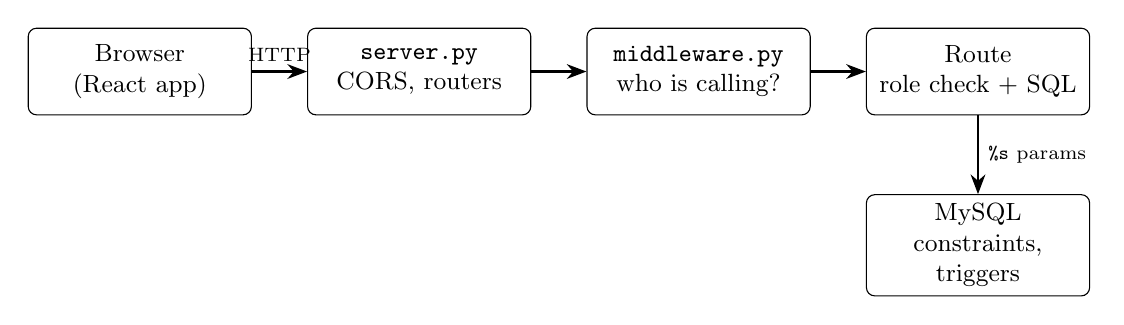
\begin{tikzpicture}[
  box/.style={draw, rounded corners=3pt, align=center, minimum height=1.1cm, text width=2.6cm, font=\small},
  arr/.style={-{Stealth[length=2.5mm]}, thick}
]
\node[box] (b) {Browser\\(React app)};
\node[box, right=0.7cm of b] (s) {\code{server.py}\\CORS, routers};
\node[box, right=0.7cm of s] (m) {\code{middleware.py}\\who is calling?};
\node[box, right=0.7cm of m] (r) {Route\\role check + SQL};
\node[box, below=1.0cm of r] (d) {MySQL\\constraints, triggers};
\draw[arr] (b) -- node[above, font=\scriptsize] {HTTP} (s);
\draw[arr] (s) -- (m);
\draw[arr] (m) -- (r);
\draw[arr] (r) -- node[right, font=\scriptsize] {\code{\%s} params} (d);
\end{tikzpicture}
\end{center}

The backend is a FastAPI application. Each request passes the CORS check in \code{server.py}, is matched to a router, and, if the route needs a login, goes through \code{getCurrentUser} in \code{middleware.py}. The route checks the caller's role, opens its own database connection, runs its SQL and closes the connection in a \code{finally} block.

\subsection{Modules}

\begin{center}
\small
\begin{tabularx}{\textwidth}{l L}
\toprule
\textbf{File} & \textbf{Responsibility} \\
\midrule
\code{server.py}      & Creates the app, loads \code{.env}, configures CORS, defines \code{getDBconnection()}, the six time slots and the 3-day booking window, and registers the routers \\
\code{middleware.py}  & \code{getCurrentUser}: hashes the bearer token and looks up an unexpired session; returns \{accountId, role, userId\} or 401 \\
\code{helpers.py}     & Password hashing and verification (scrypt with a random 16-byte salt, constant-time comparison) \\
\code{auth.py}        & Login, patient registration, current profile, logout \\
\code{patient.py}     & The patient's own profile and dashboard counts \\
\code{doctor.py}      & Departments, doctor directory and profile, free slots, medicine catalogue, the doctor's queue for today \\
\code{appointment.py} & Book, list, view, cancel, reschedule and complete appointments; maps database errors to HTTP codes \\
\code{reception.py}   & Pending bills with prescribed medicines; recording a payment \\
\bottomrule
\end{tabularx}
\end{center}

\subsection{Endpoints}

\begin{center}
\footnotesize
\begin{tabularx}{\textwidth}{l l l L}
\toprule
\textbf{Method} & \textbf{Path} & \textbf{Caller} & \textbf{Purpose} \\
\midrule
GET    & \code{/health/db}                        & anyone     & Database connectivity check \\
POST   & \code{/auth/login}                       & anyone     & Log in, returns token and profile \\
POST   & \code{/auth/register}                    & anyone     & Patient self-registration \\
GET    & \code{/auth/me}                          & logged in  & Current profile \\
DELETE & \code{/auth/session}                     & logged in  & Log out \\
GET    & \code{/patients/me}                      & patient    & Own details \\
GET    & \code{/patients/me/dashboard}            & patient    & Upcoming visits, unpaid bills, running prescriptions \\
GET    & \code{/patients/me/appointments}         & patient    & All own visits with prescription and bill \\
GET    & \code{/departments}                      & anyone     & Department list \\
GET    & \code{/doctors}                          & anyone     & Active doctors, optional department filter \\
GET    & \code{/doctors/\{id\}}                   & anyone     & Doctor profile \\
GET    & \code{/doctors/\{id\}/slots?date=}       & anyone     & Free slots on a date \\
GET    & \code{/medicines}                        & logged in  & Medicine catalogue \\
GET    & \code{/doctors/me/appointments}          & doctor     & Today's queue \\
POST   & \code{/appointments}                     & patient    & Book \\
GET    & \code{/appointments/\{id\}}              & its patient or doctor & Visit details; doctors also get patient history \\
PATCH  & \code{/appointments/\{id\}/cancel}       & patient    & Cancel \\
PATCH  & \code{/appointments/\{id\}/reschedule}   & patient    & Reschedule \\
POST   & \code{/appointments/\{id\}/complete}     & doctor     & Prescription + bill \\
GET    & \code{/reception/pending-bills}          & pharmacist & Unpaid bills with medicines \\
POST   & \code{/bills/\{id\}/payments}            & pharmacist & Record payment \\
\bottomrule
\end{tabularx}
\end{center}

\subsection{Authentication and errors}

\begin{itemize}
  \item \textbf{Passwords} are stored as \code{scrypt\$<salt>\$<hash>} ($n = 16384$, $r = 8$, $p = 1$). scrypt is deliberately slow, so a stolen hash is expensive to guess.
  \item \textbf{Sessions}: login creates a random token (\code{secrets.token\_urlsafe(32)}), valid for one day. The client sends it as \code{Authorization: Bearer <token>}; the server stores and compares only its SHA-256 hash.
  \item \textbf{Authorisation}: every protected route checks the caller's role (403 otherwise), and reads the patient or doctor ID from the session, never from the URL, so users can only see their own records.
  \item \textbf{Error mapping}: duplicate key (1062) $\Rightarrow$ 409 ``slot already occupied''; trigger \code{SIGNAL} (SQLSTATE 45000) $\Rightarrow$ 409 with the trigger's message; anything else $\Rightarrow$ 500.
  \item \textbf{Time}: all ``today'' checks in Python use Asia/Kolkata time.
\end{itemize}

% ============================================================== 11
\section{Frontend}

\subsection{Overview}

The frontend is a single-page React 19 application built with Vite, styled with Tailwind CSS, routed with React Router and using Lucide icons. It shows only the workflows the backend supports, so no button promises something the server cannot do.

\begin{itemize}
  \item \code{src/api/client.js} is the only place that calls the server. It adds the bearer token (kept in \code{sessionStorage}) and turns error responses into readable messages; a 401 sends the user back to the login page.
  \item \code{src/api/normalize.js} maps database column names to the shapes the screens use, and converts rupees to integer paise to avoid rounding errors.
  \item \code{src/pages/} holds one folder per area (overview, appointments, doctors, prescriptions, billing); \code{src/components/} holds shared parts such as the app shell, data tables, dialogs and the slot picker.
  \item Each route renders a different screen per role, and a role with no screen for a route sees ``access denied''.
  \item \code{npm test} runs 18 tests of the booking rules and the API contract.
\end{itemize}

\begin{center}
\small
\begin{tabularx}{\textwidth}{l L L L}
\toprule
\textbf{Route} & \textbf{Patient} & \textbf{Doctor} & \textbf{Pharmacist} \\
\midrule
\code{/overview}          & Dashboard & Today's numbers & Pending-bill numbers \\
\code{/appointments}      & Own visits by tab, reschedule, cancel & Today's queue & -- \\
\code{/appointments/:id}  & Visit, prescription, bill & Patient details, history, complete visit & -- \\
\code{/doctors}, \code{/doctors/:id} & Directory, slots, booking & -- & -- \\
\code{/prescriptions}     & Running and past prescriptions & -- & -- \\
\code{/billing}, \code{/billing/:id} & Own bills & -- & Pending bills, record payment \\
\code{/settings}          & Profile & Profile & Profile \\
\bottomrule
\end{tabularx}
\end{center}

\subsection{Screenshots}

The screenshots below were taken from the running application with the seed data loaded.

\begin{figure}[H]
\centering
\begin{subfigure}{0.49\textwidth}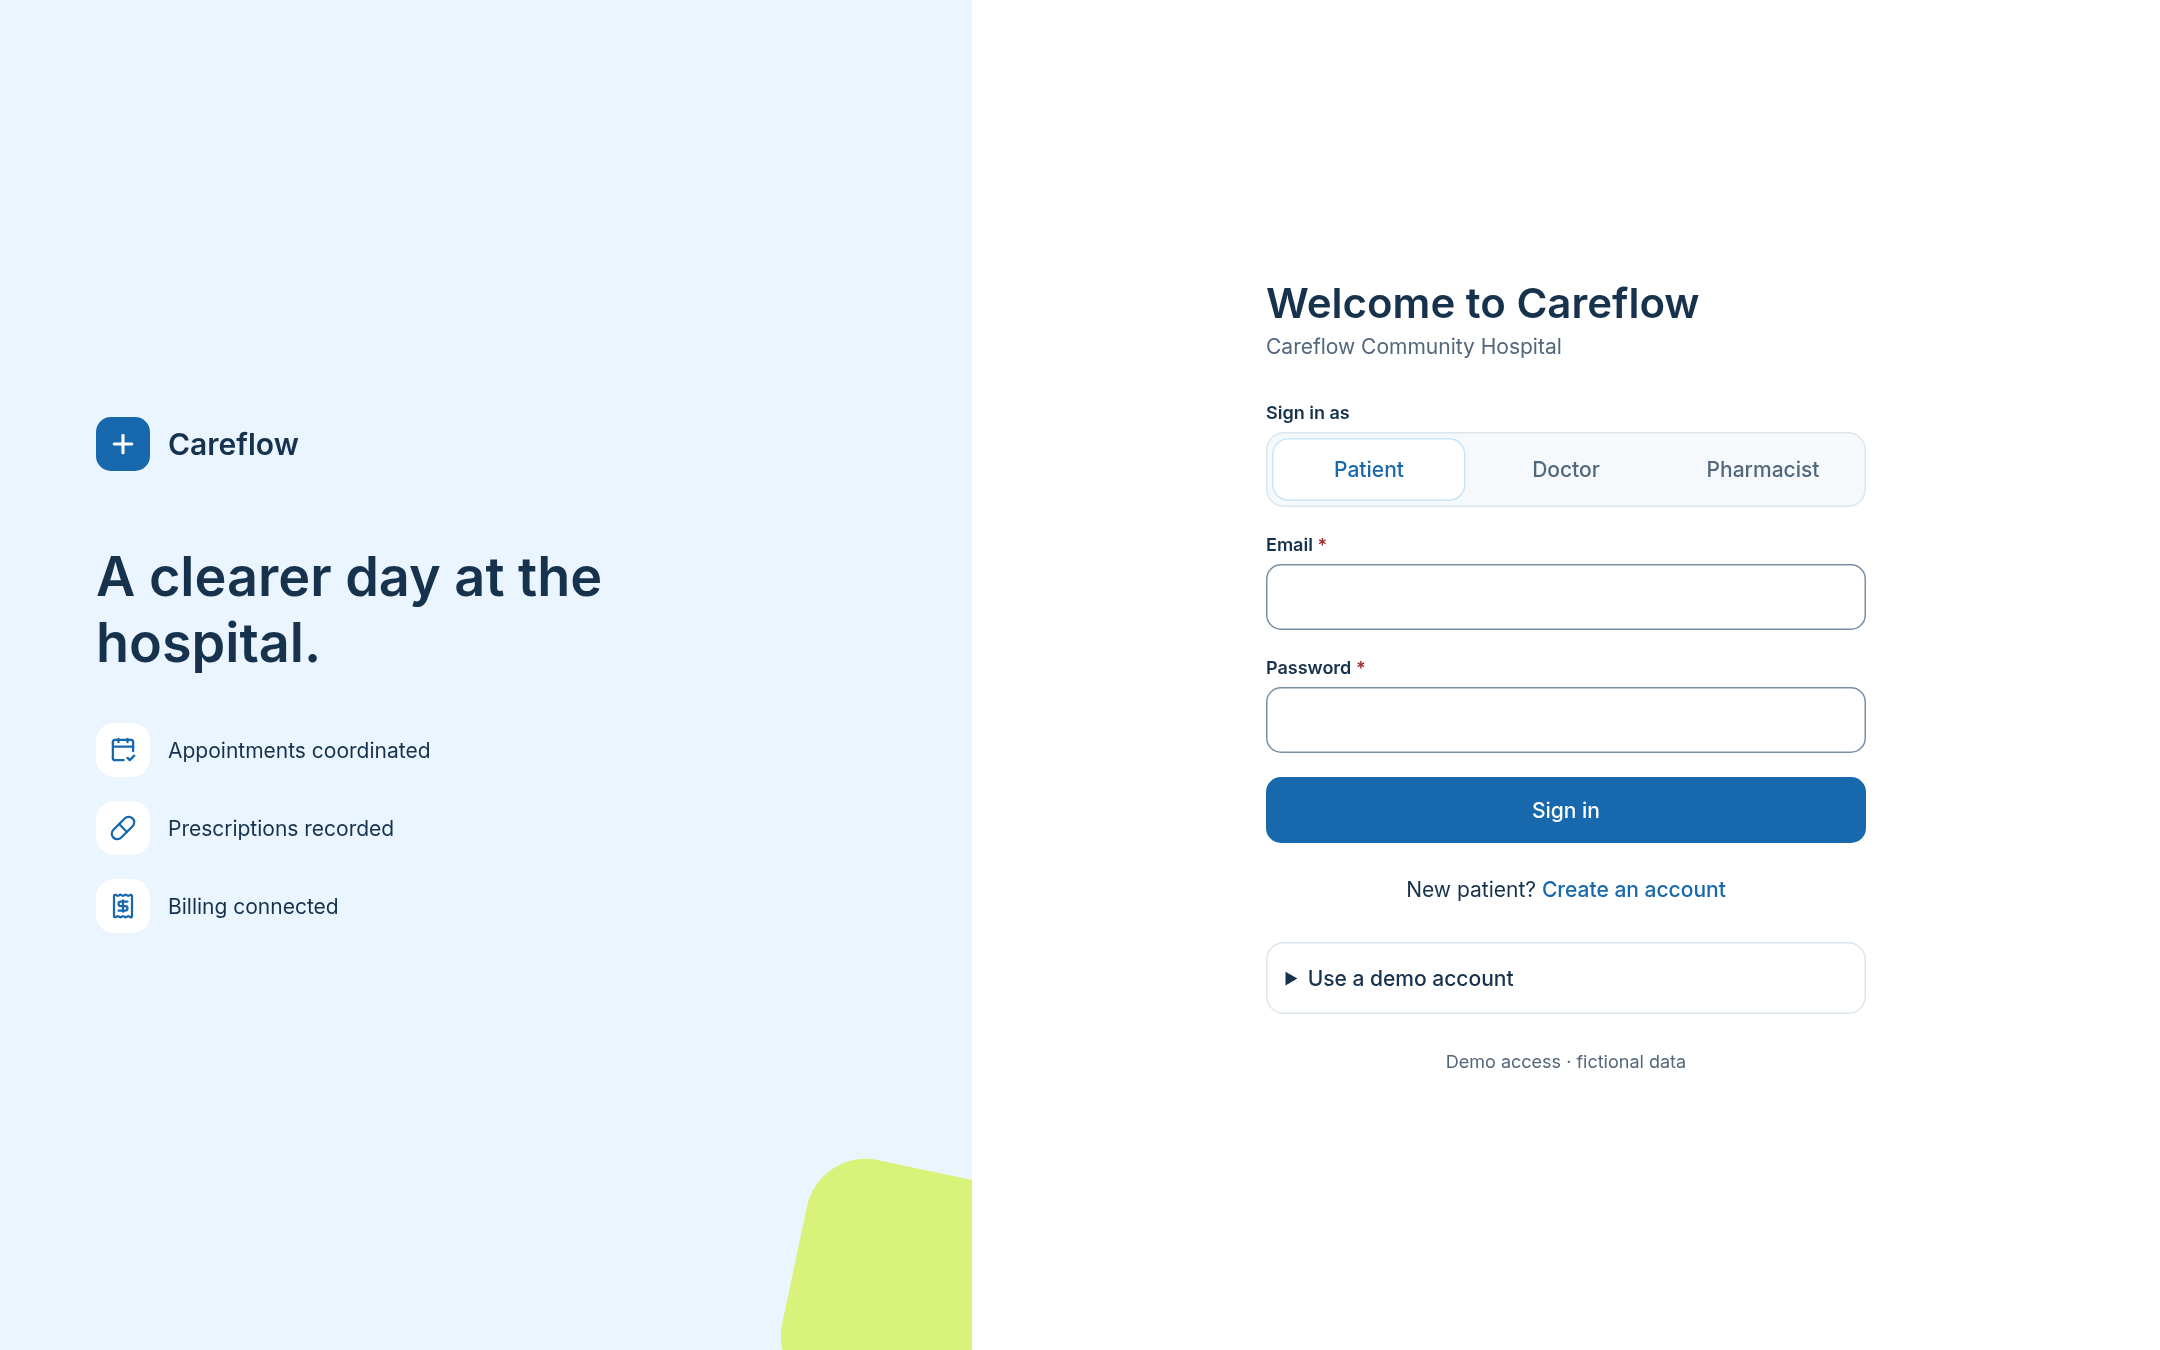
\includegraphics[width=\linewidth]{screenshots/01-login.png}\caption{Sign in, with a role picker}\end{subfigure}\hfill
\begin{subfigure}{0.49\textwidth}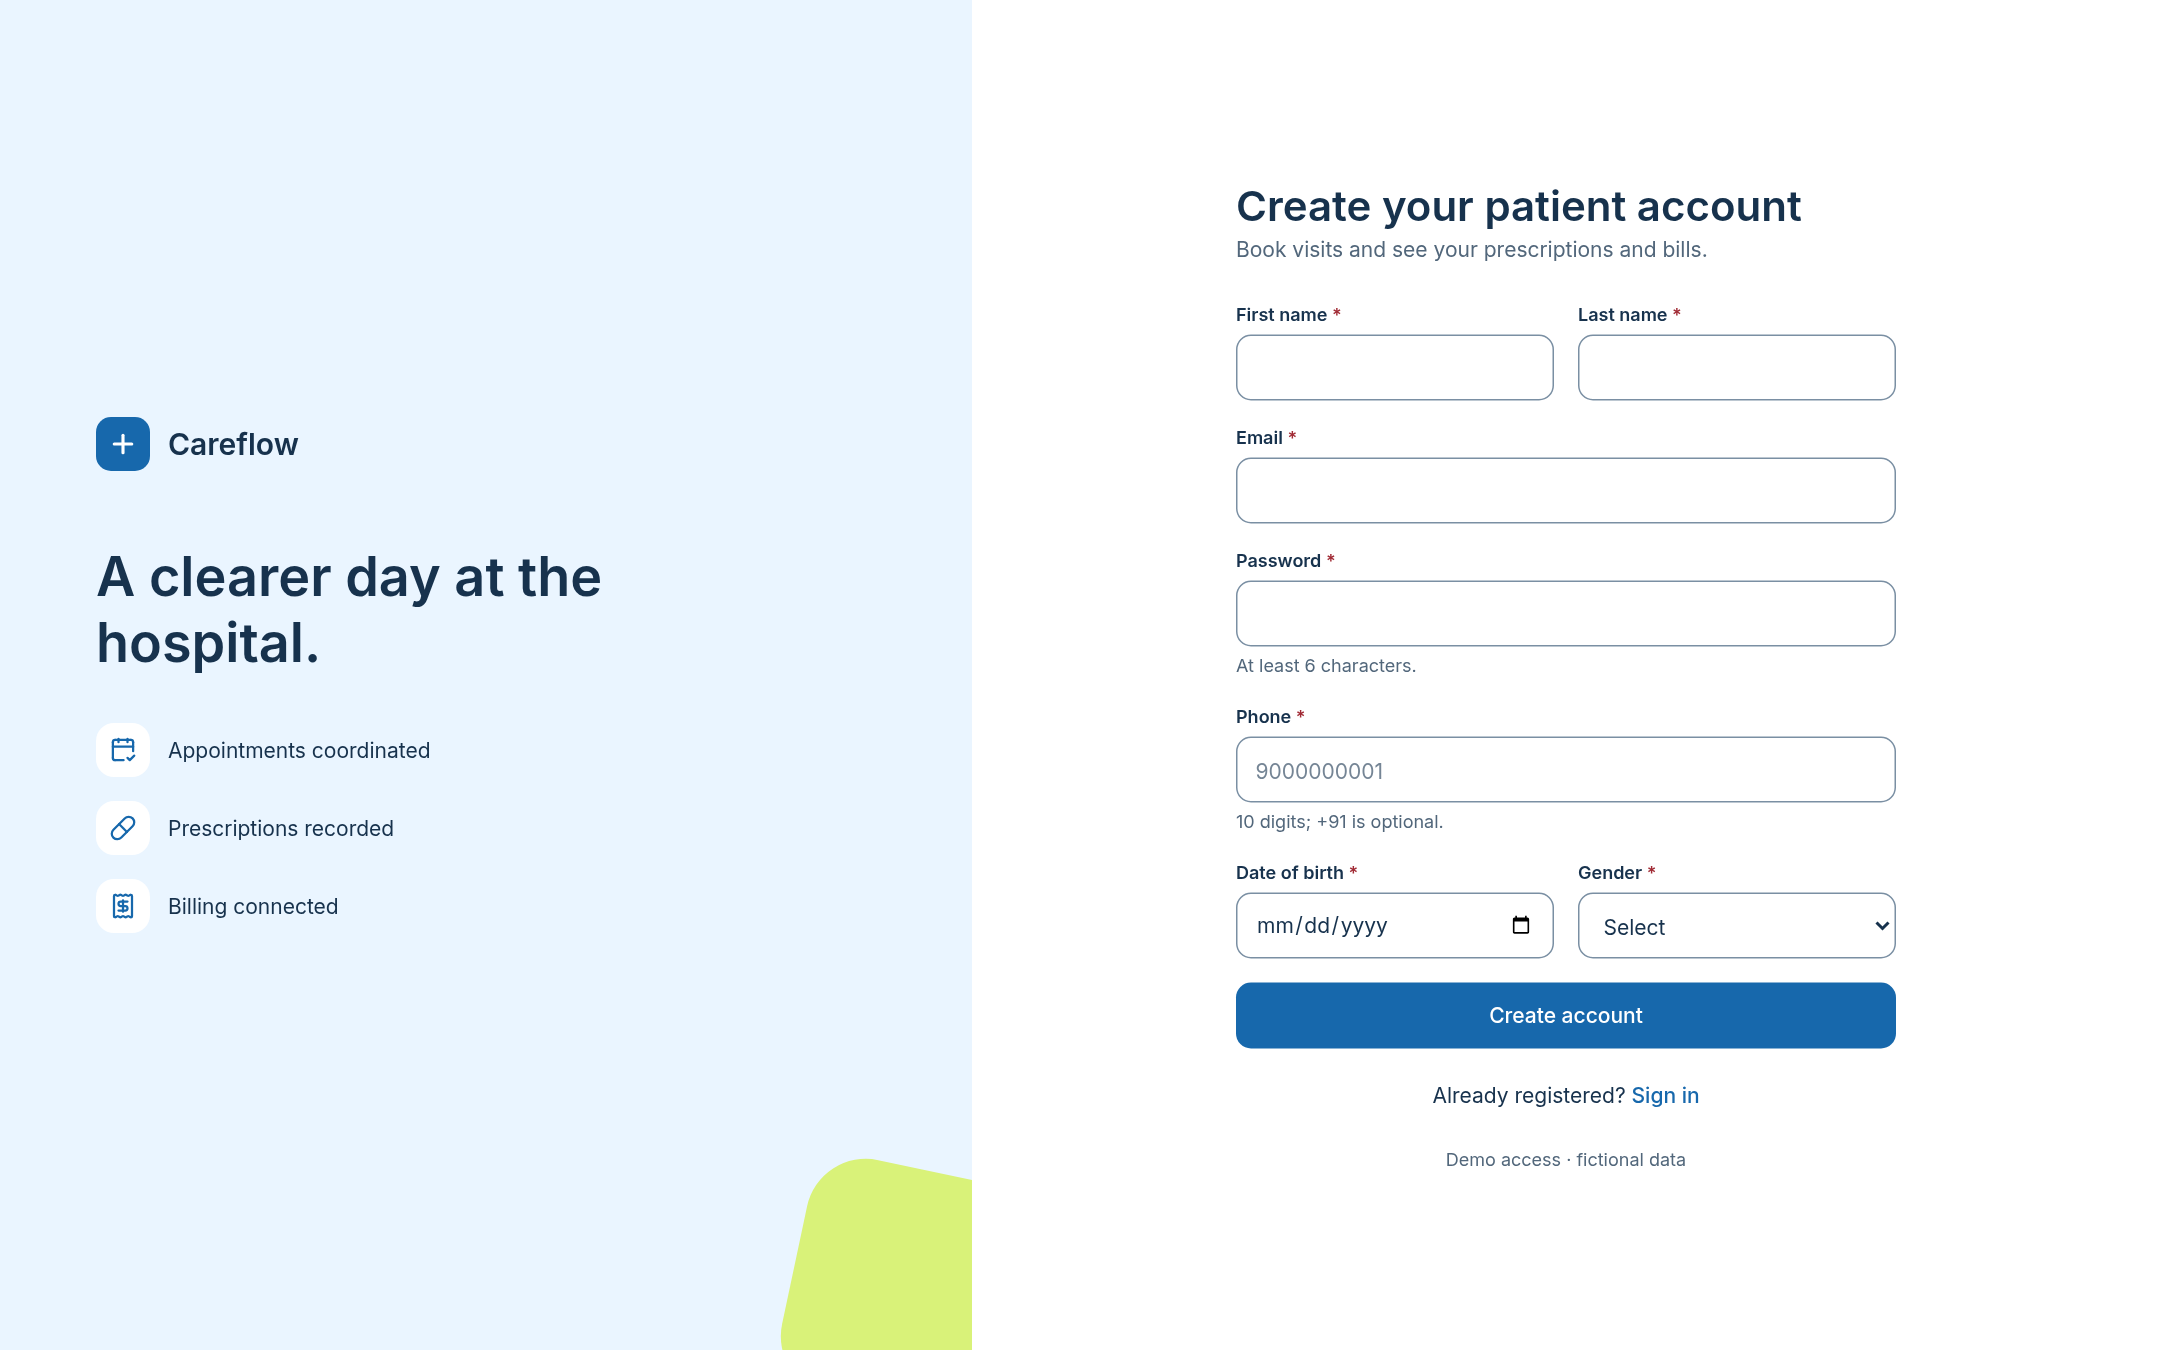
\includegraphics[width=\linewidth]{screenshots/02-register.png}\caption{Patient registration}\end{subfigure}
\caption{Public pages}
\end{figure}

\begin{figure}[H]
\centering
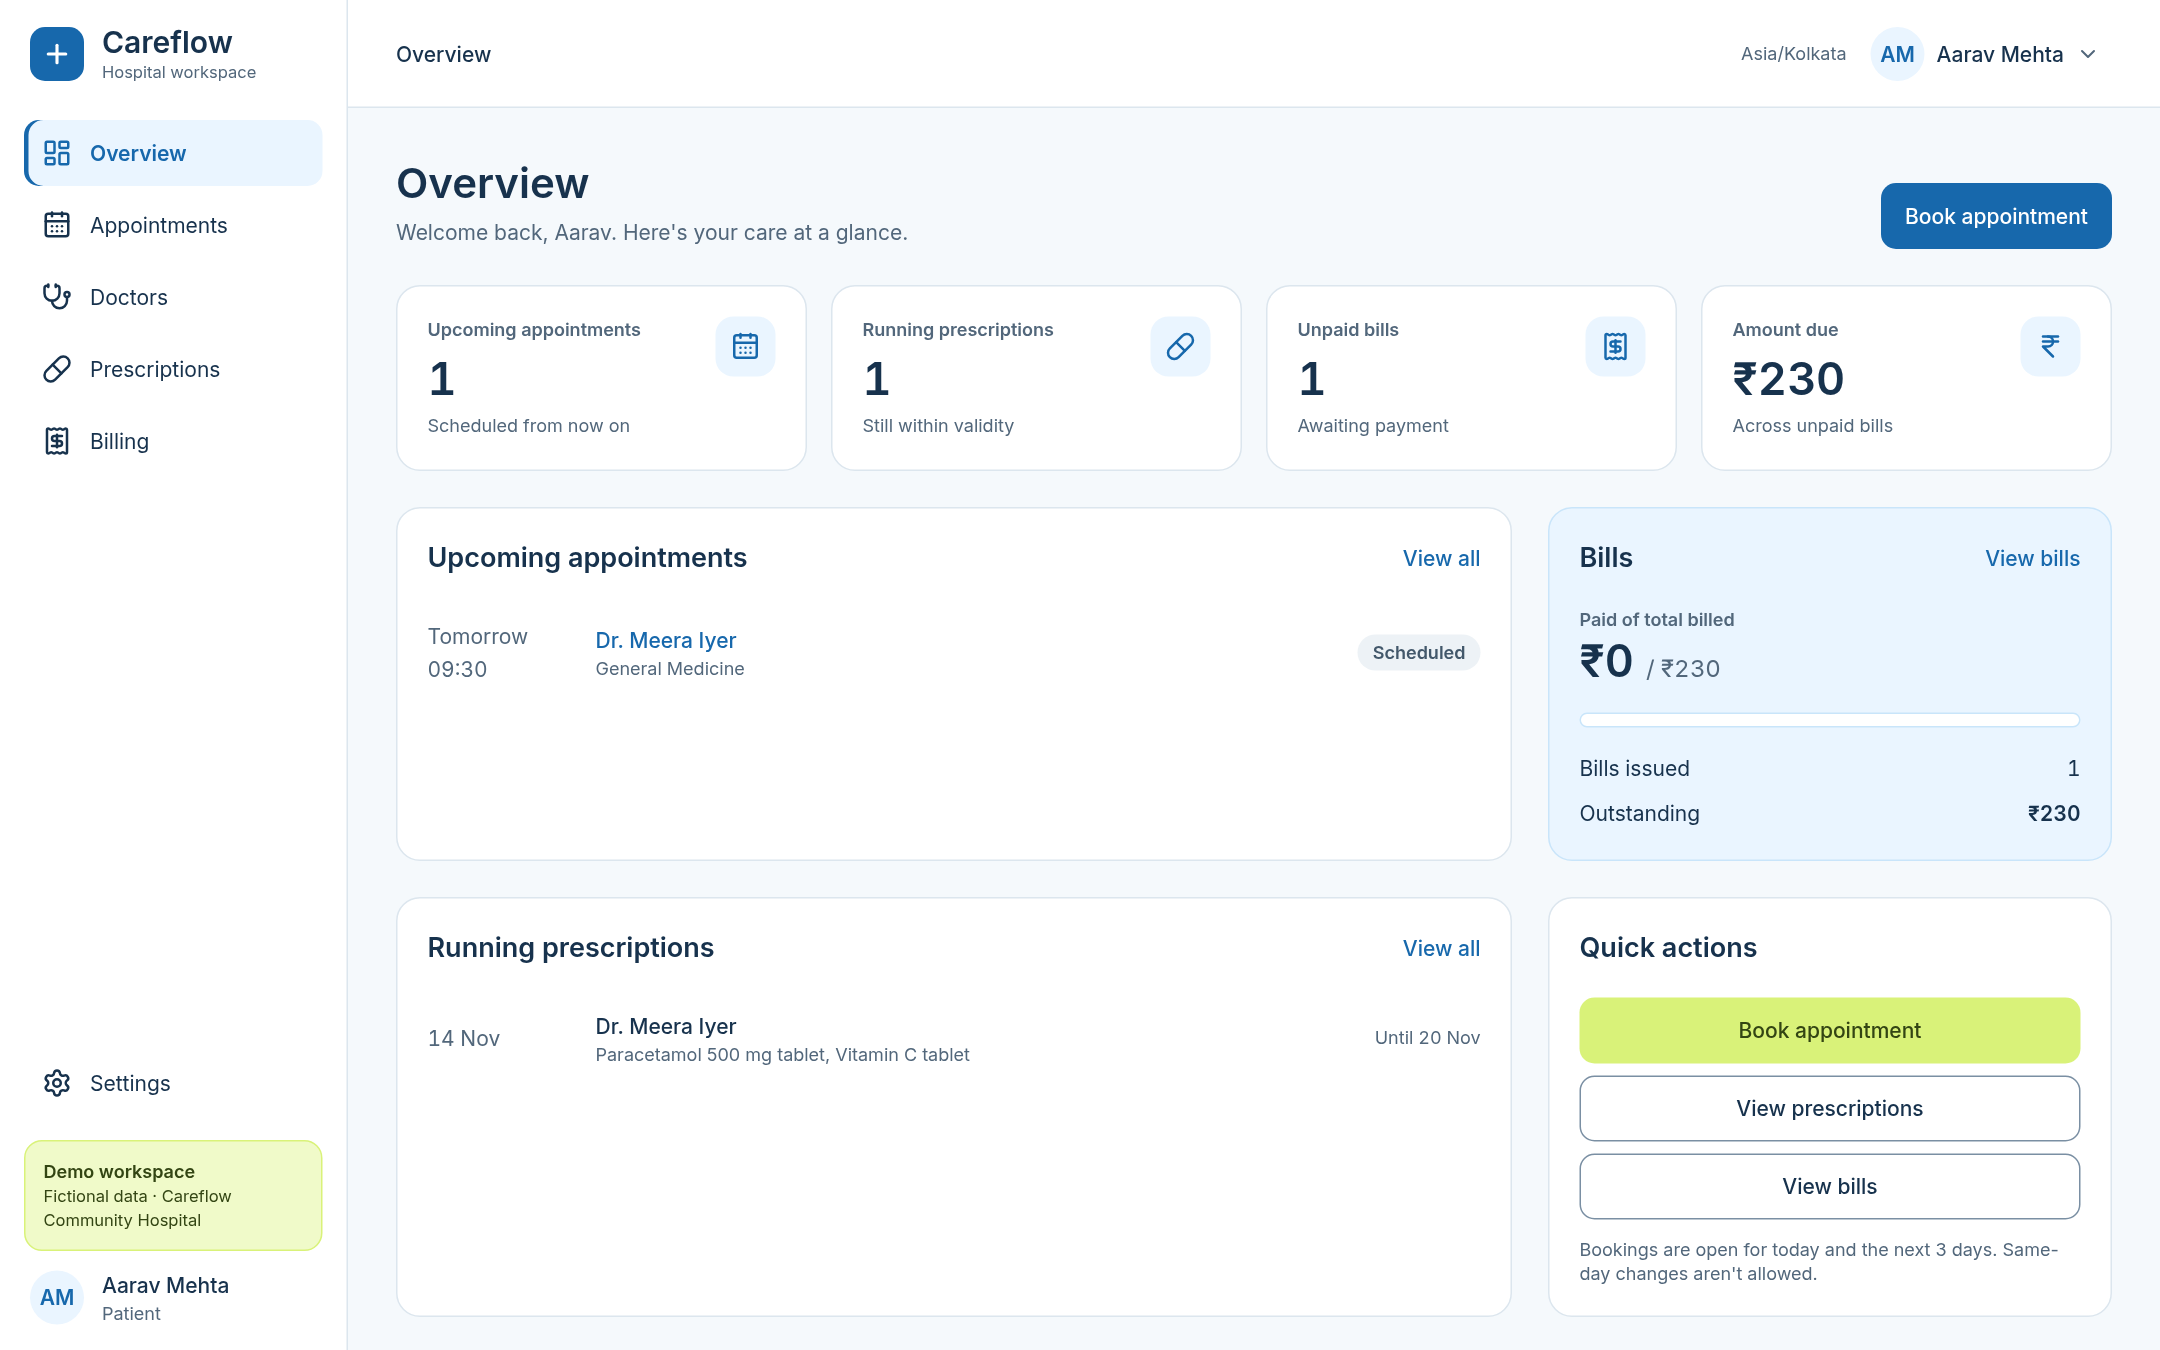
\includegraphics[width=0.9\textwidth]{screenshots/03-patient-overview.png}
\caption{Patient overview: upcoming visits, running prescriptions and amount due}
\end{figure}

\begin{figure}[H]
\centering
\begin{subfigure}{0.49\textwidth}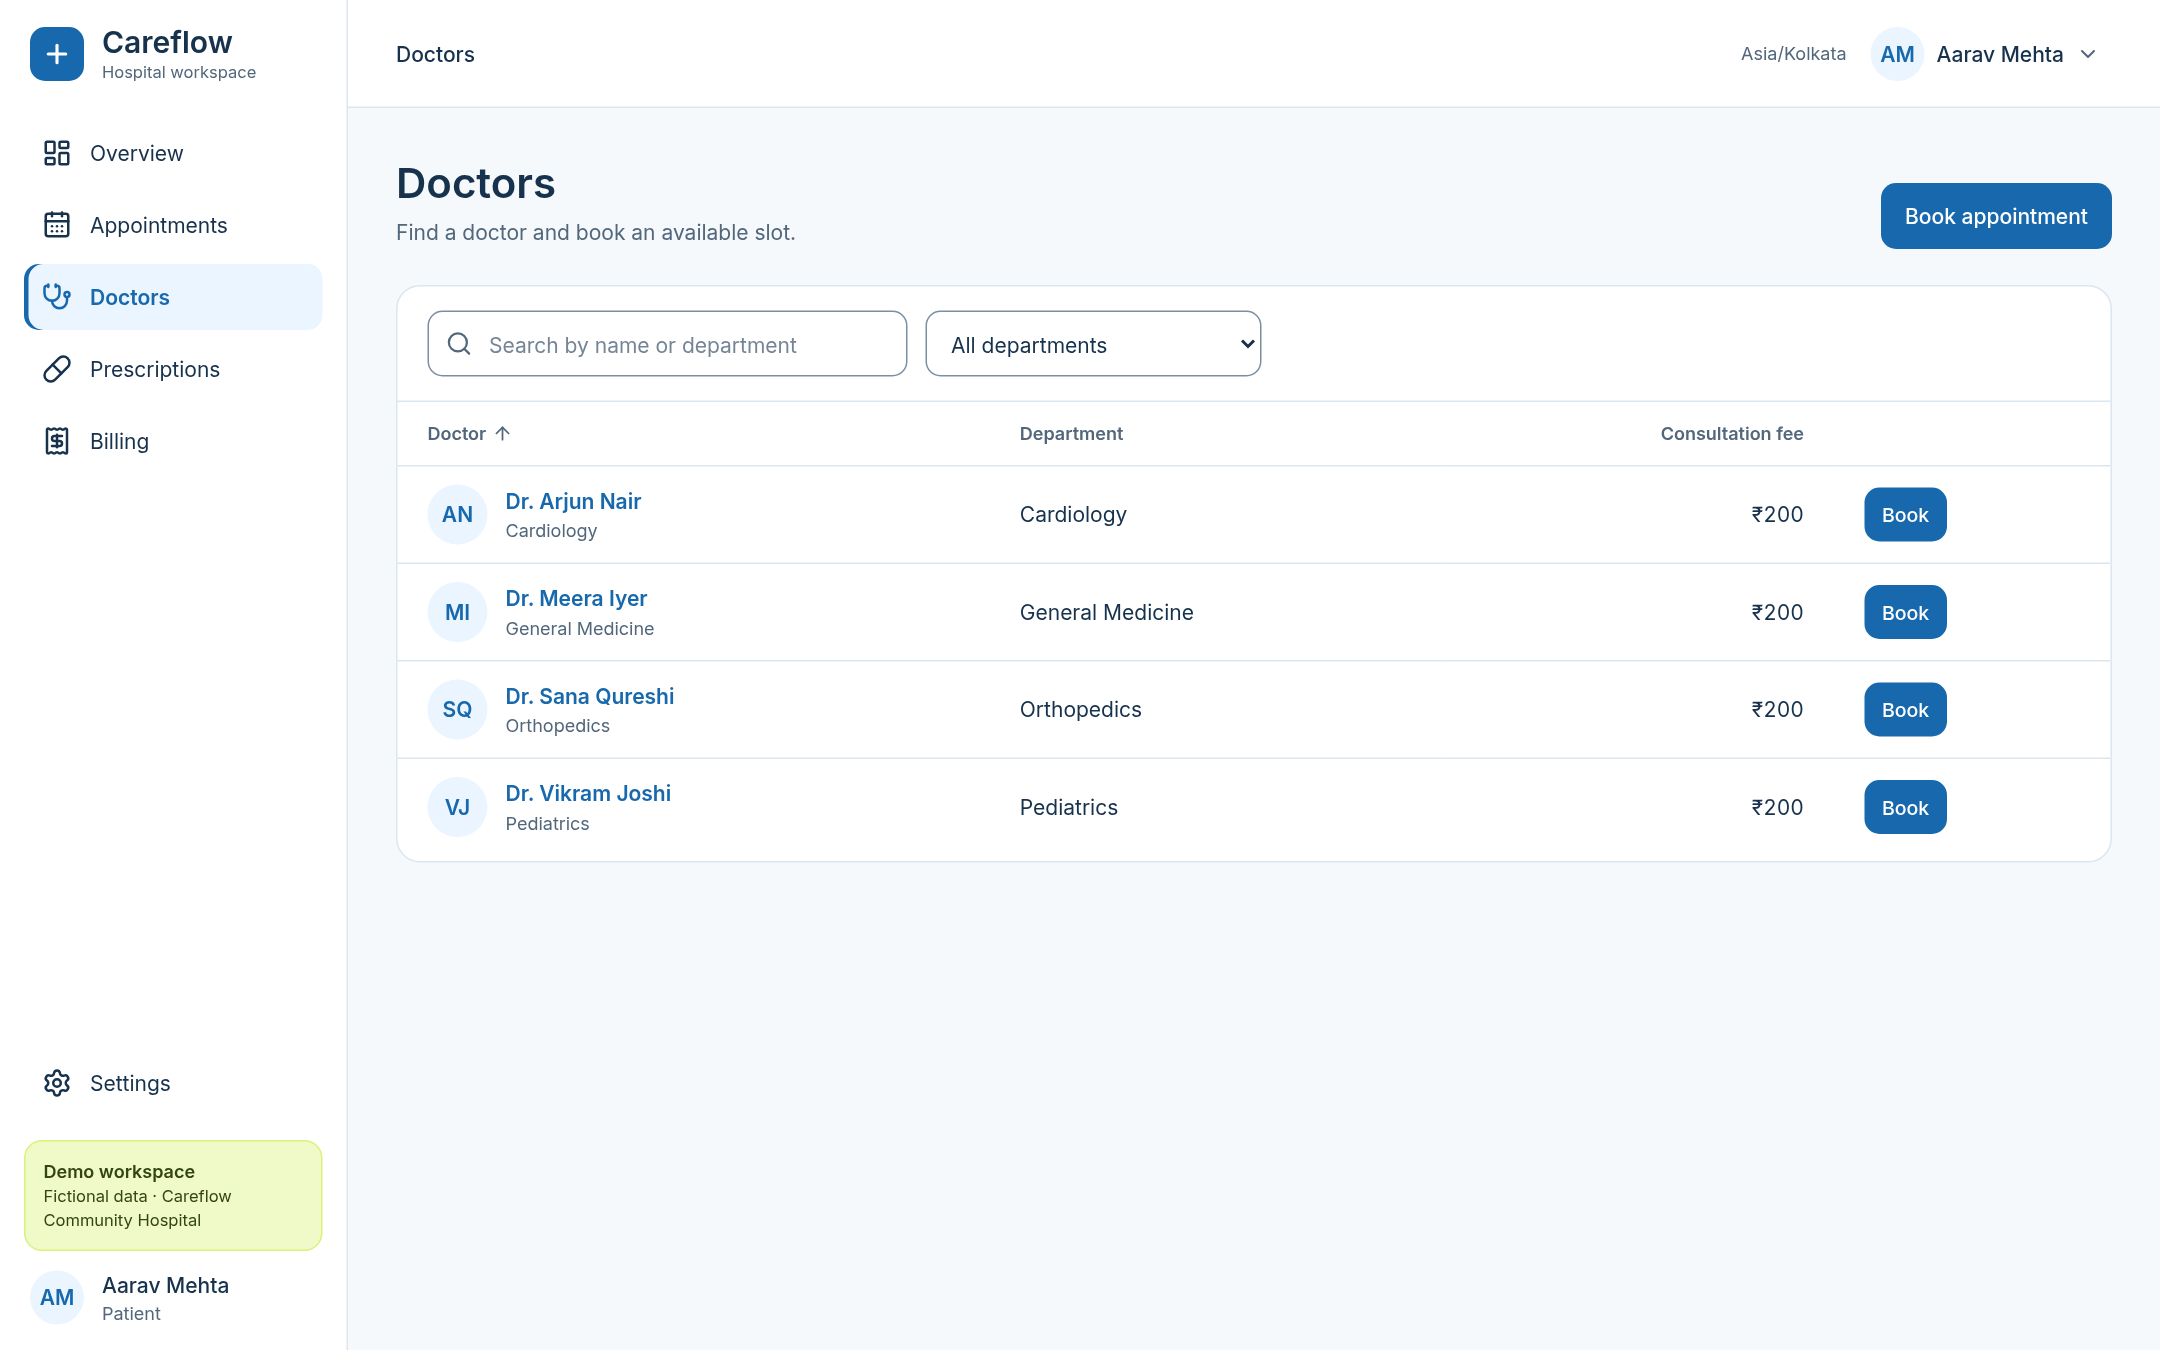
\includegraphics[width=\linewidth]{screenshots/04-doctors.png}\caption{Doctor directory}\end{subfigure}\hfill
\begin{subfigure}{0.49\textwidth}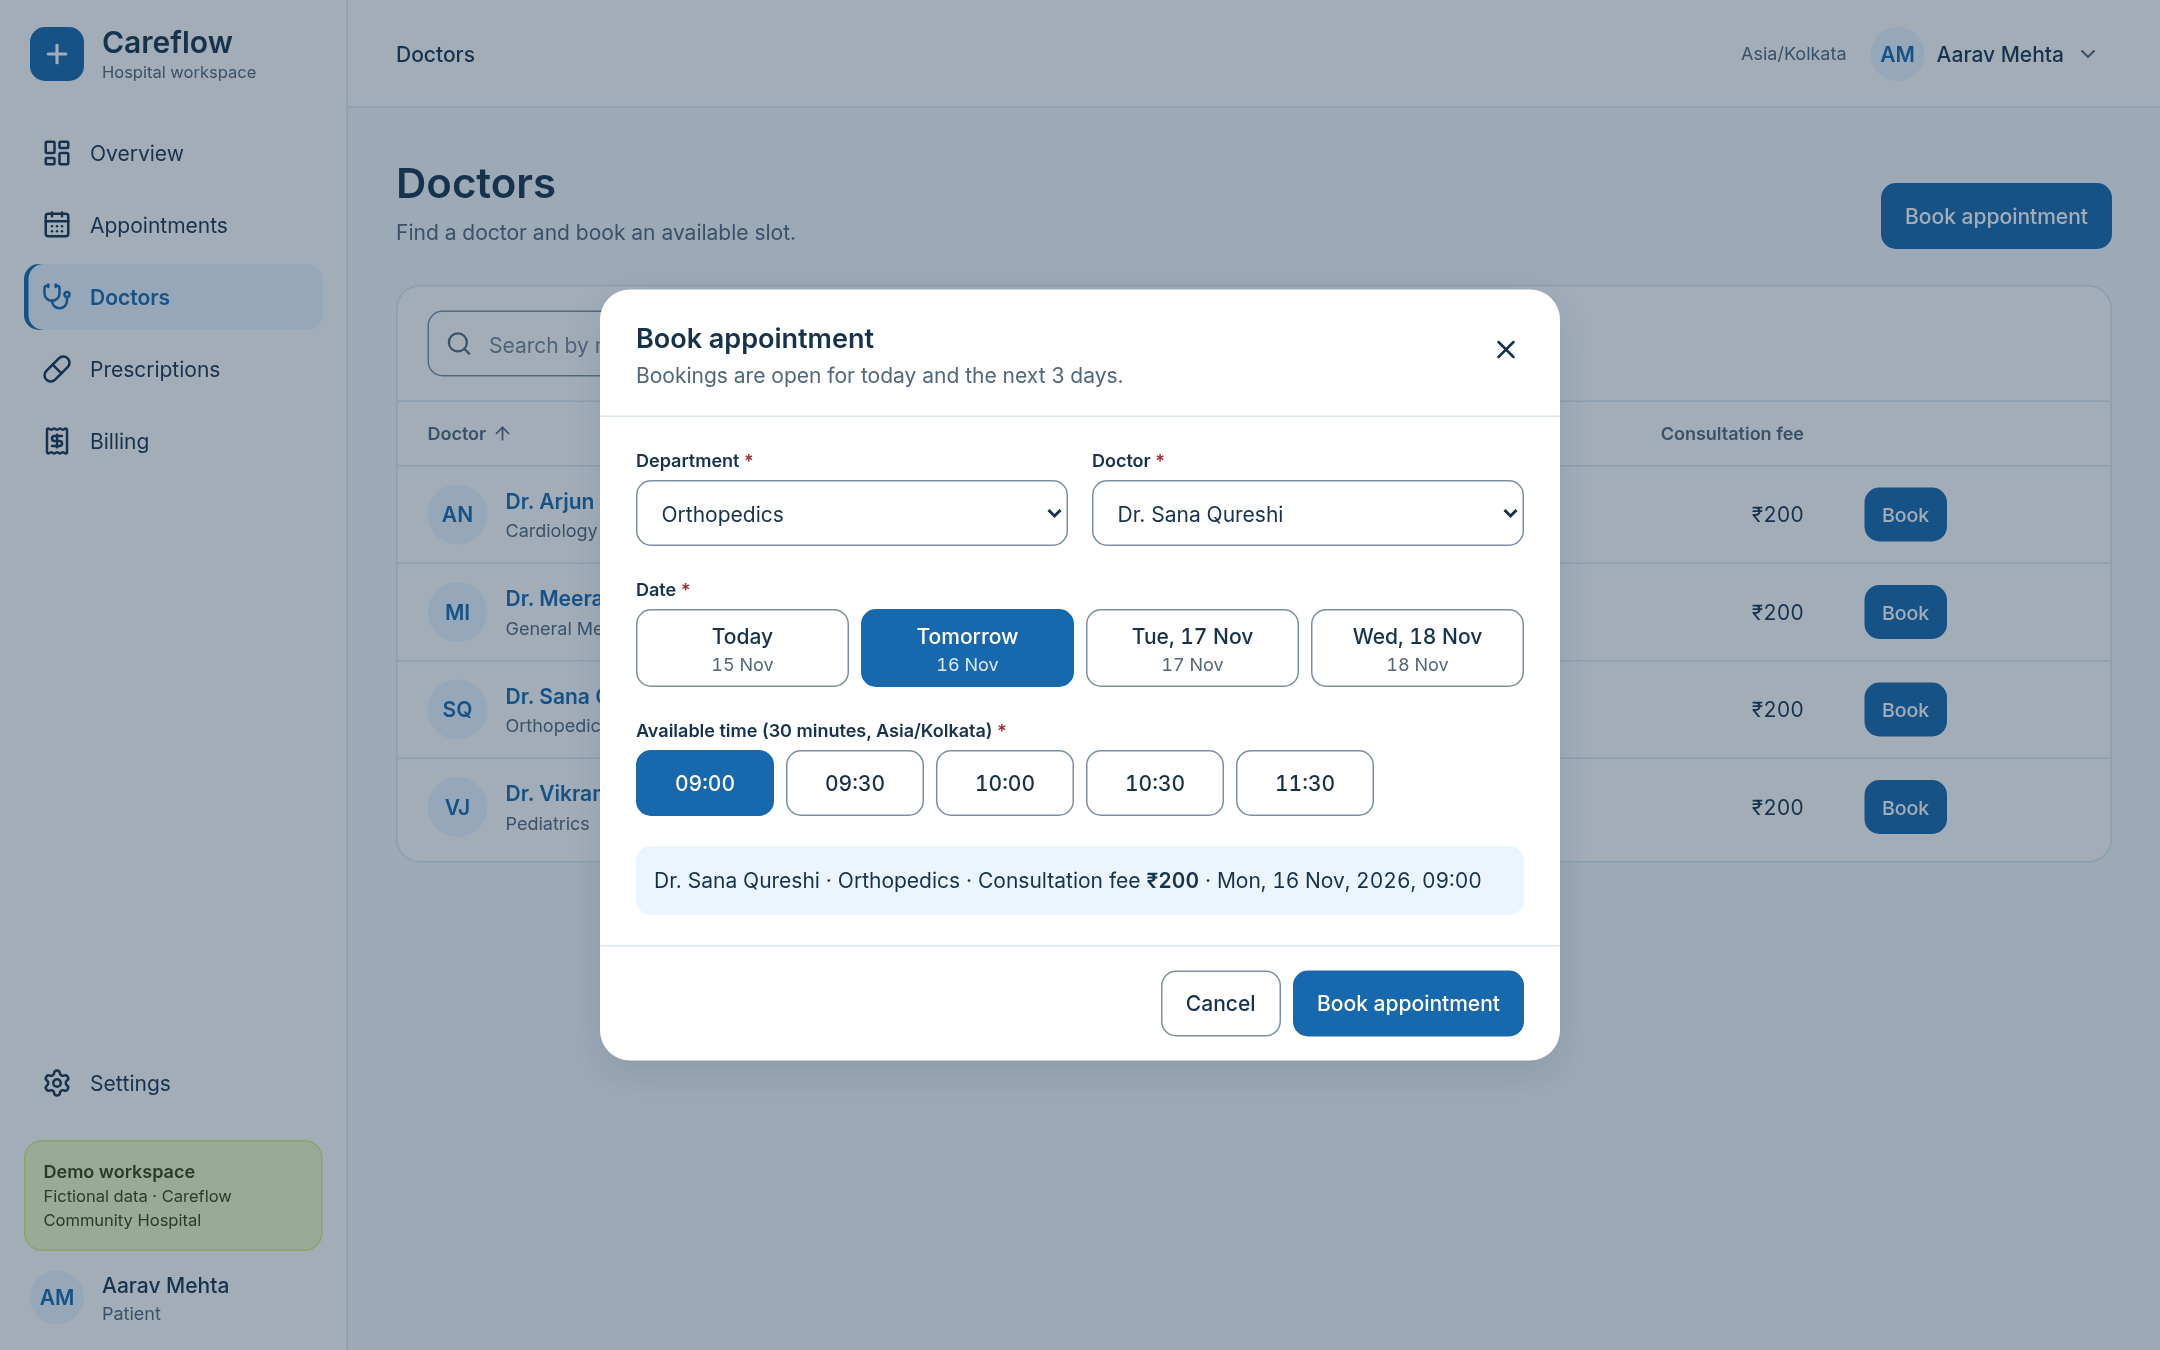
\includegraphics[width=\linewidth]{screenshots/05-booking.png}\caption{Booking dialog with free slots}\end{subfigure}
\caption{Finding a doctor and booking}
\end{figure}

\begin{figure}[H]
\centering
\begin{subfigure}{0.49\textwidth}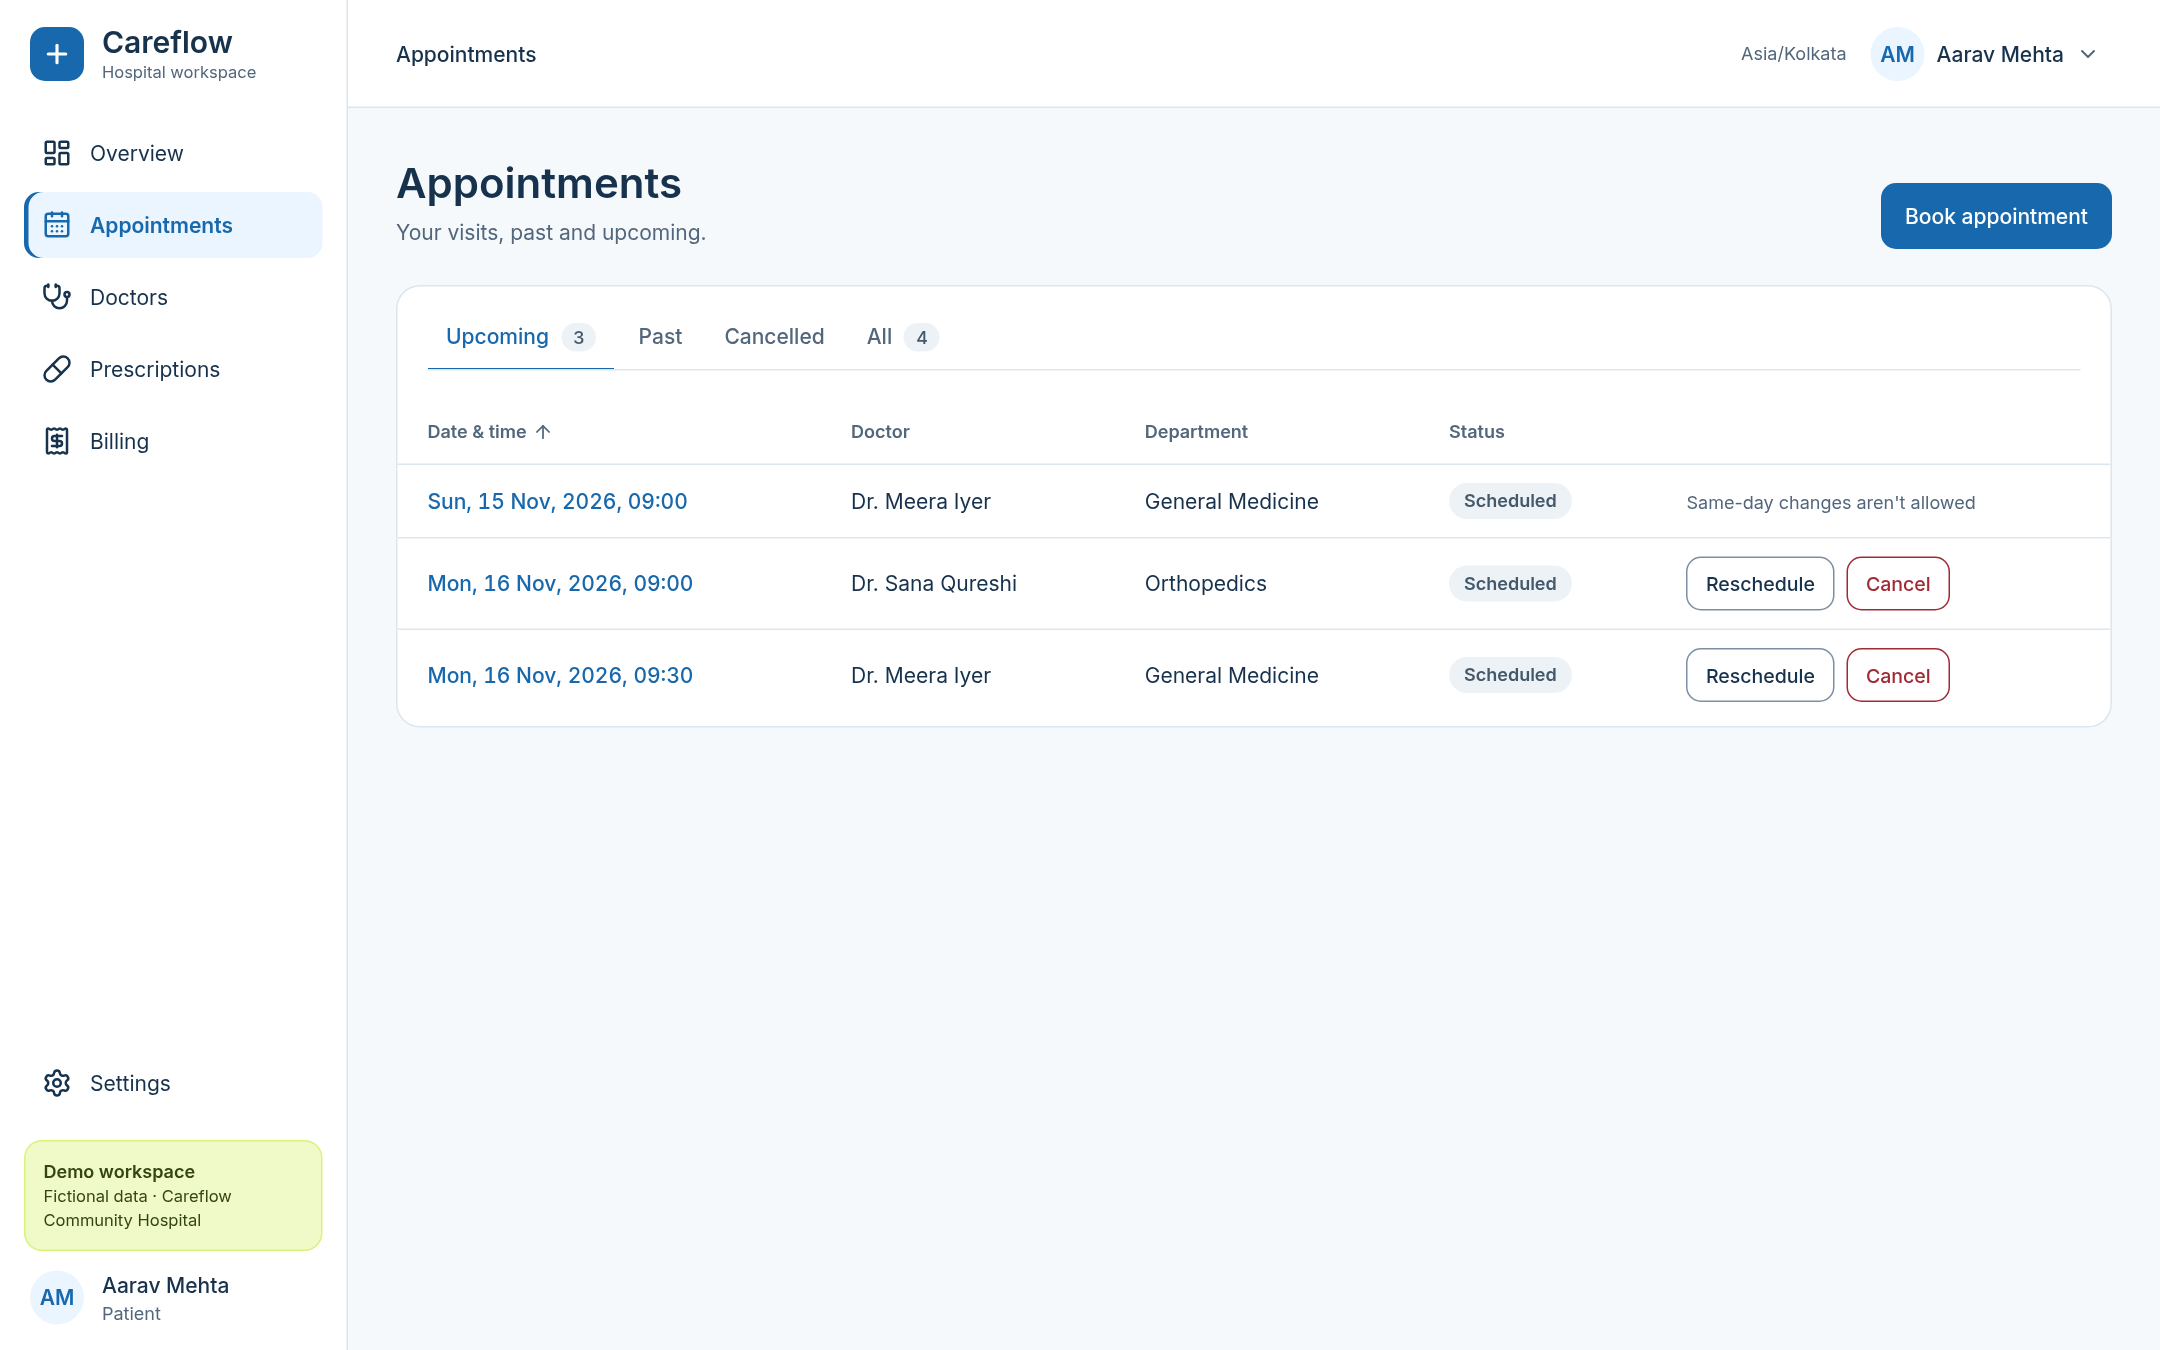
\includegraphics[width=\linewidth]{screenshots/06-appointments.png}\caption{Appointment list}\end{subfigure}\hfill
\begin{subfigure}{0.49\textwidth}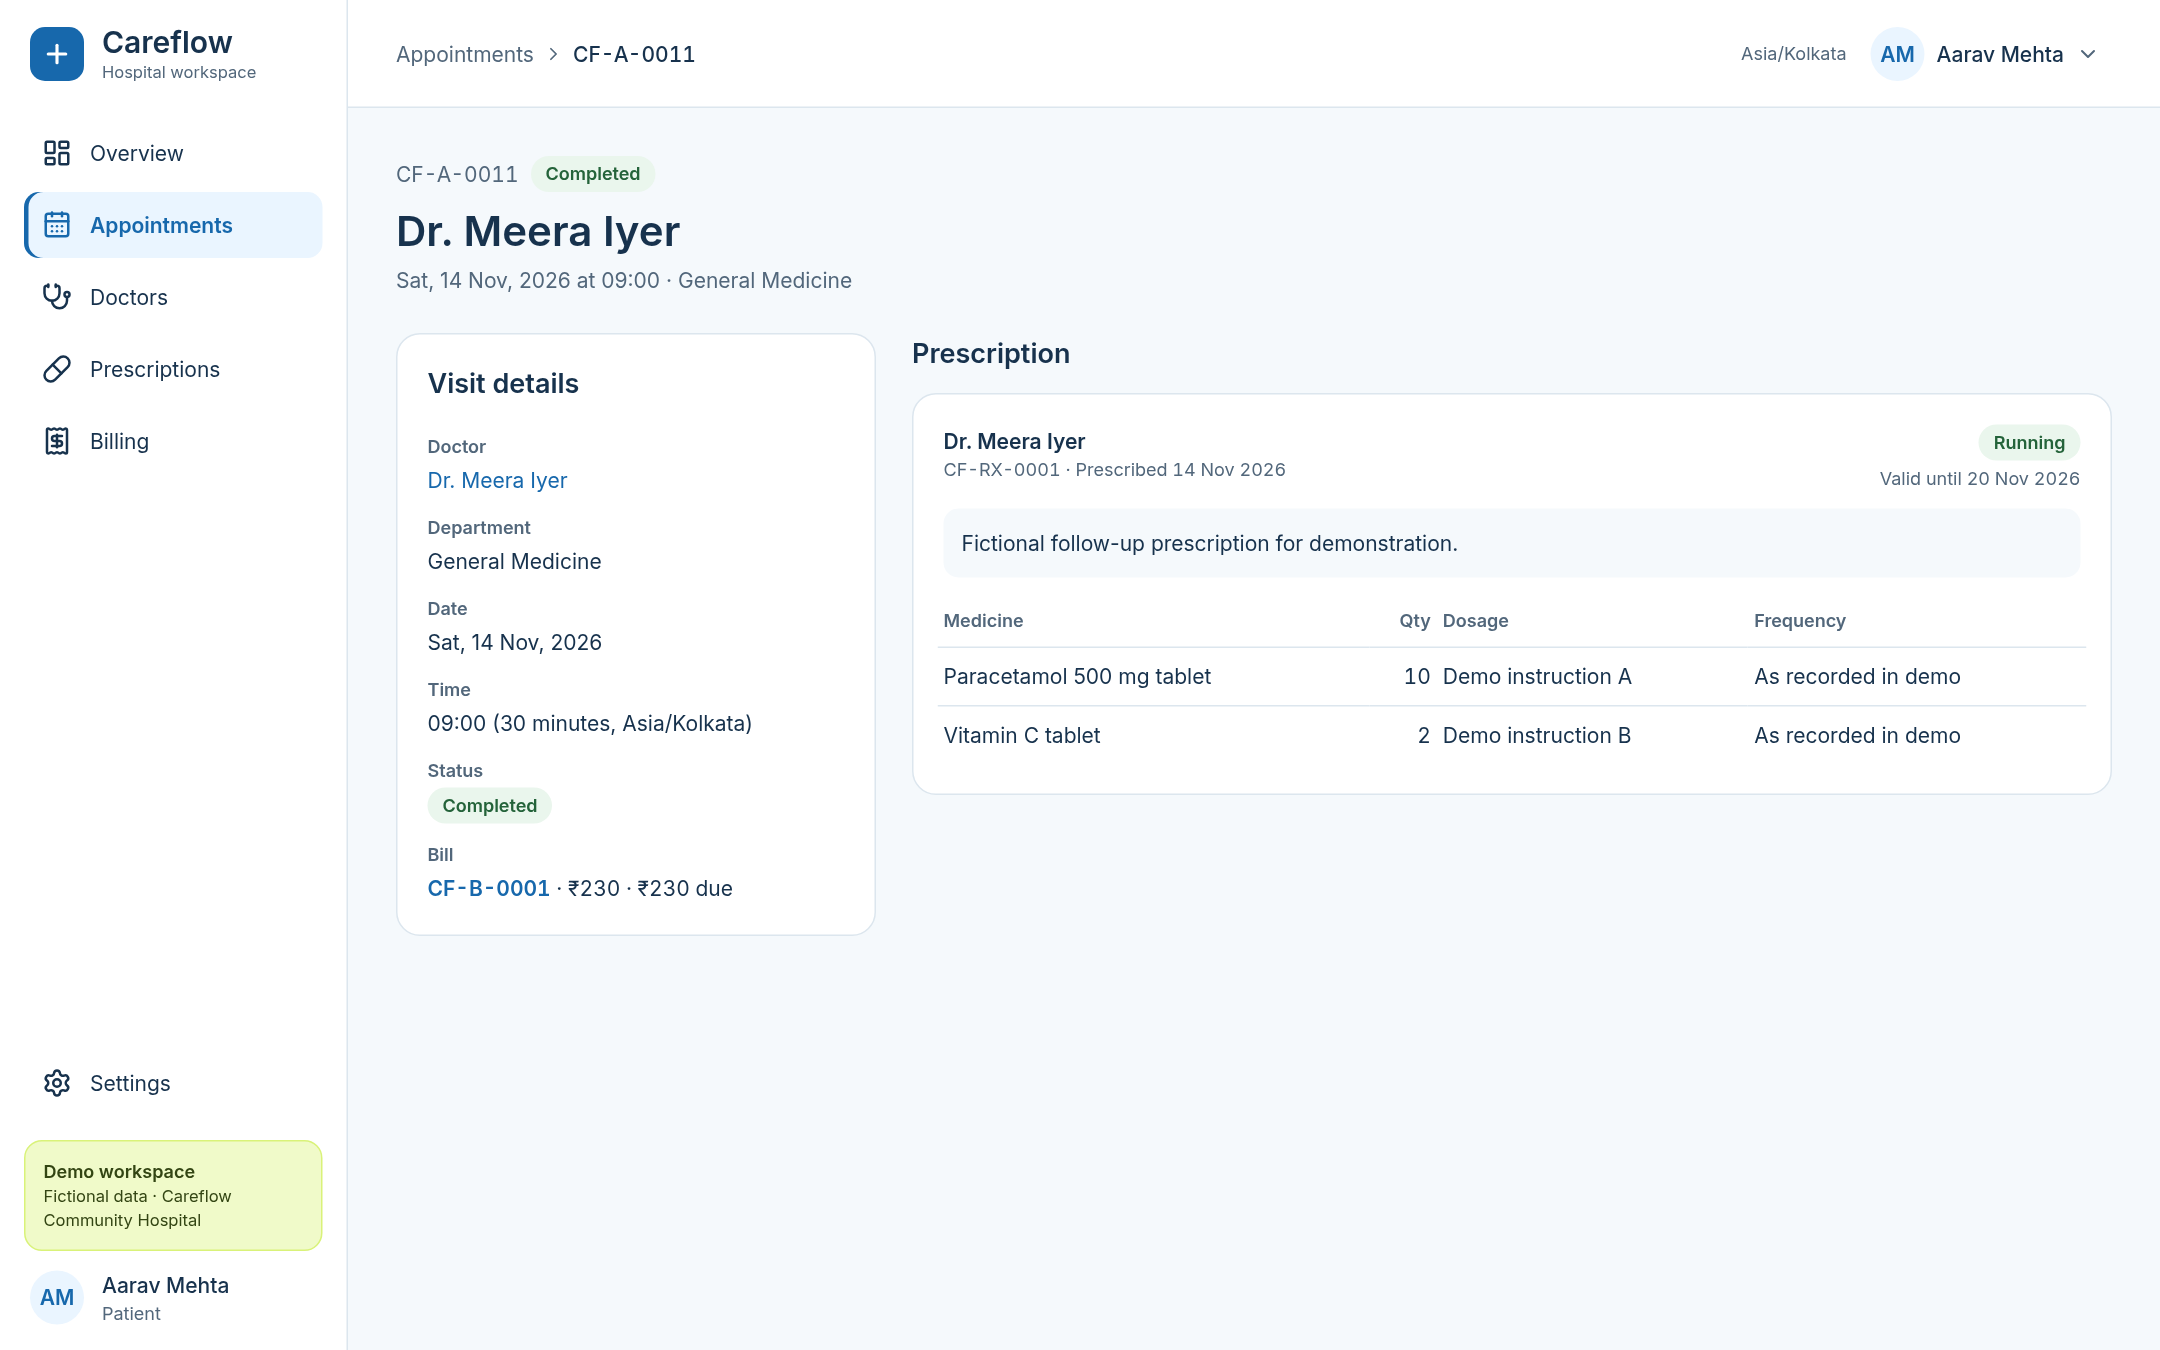
\includegraphics[width=\linewidth]{screenshots/07-visit-detail.png}\caption{A completed visit with its prescription}\end{subfigure}
\caption{Patient appointments}
\end{figure}

\begin{figure}[H]
\centering
\begin{subfigure}{0.49\textwidth}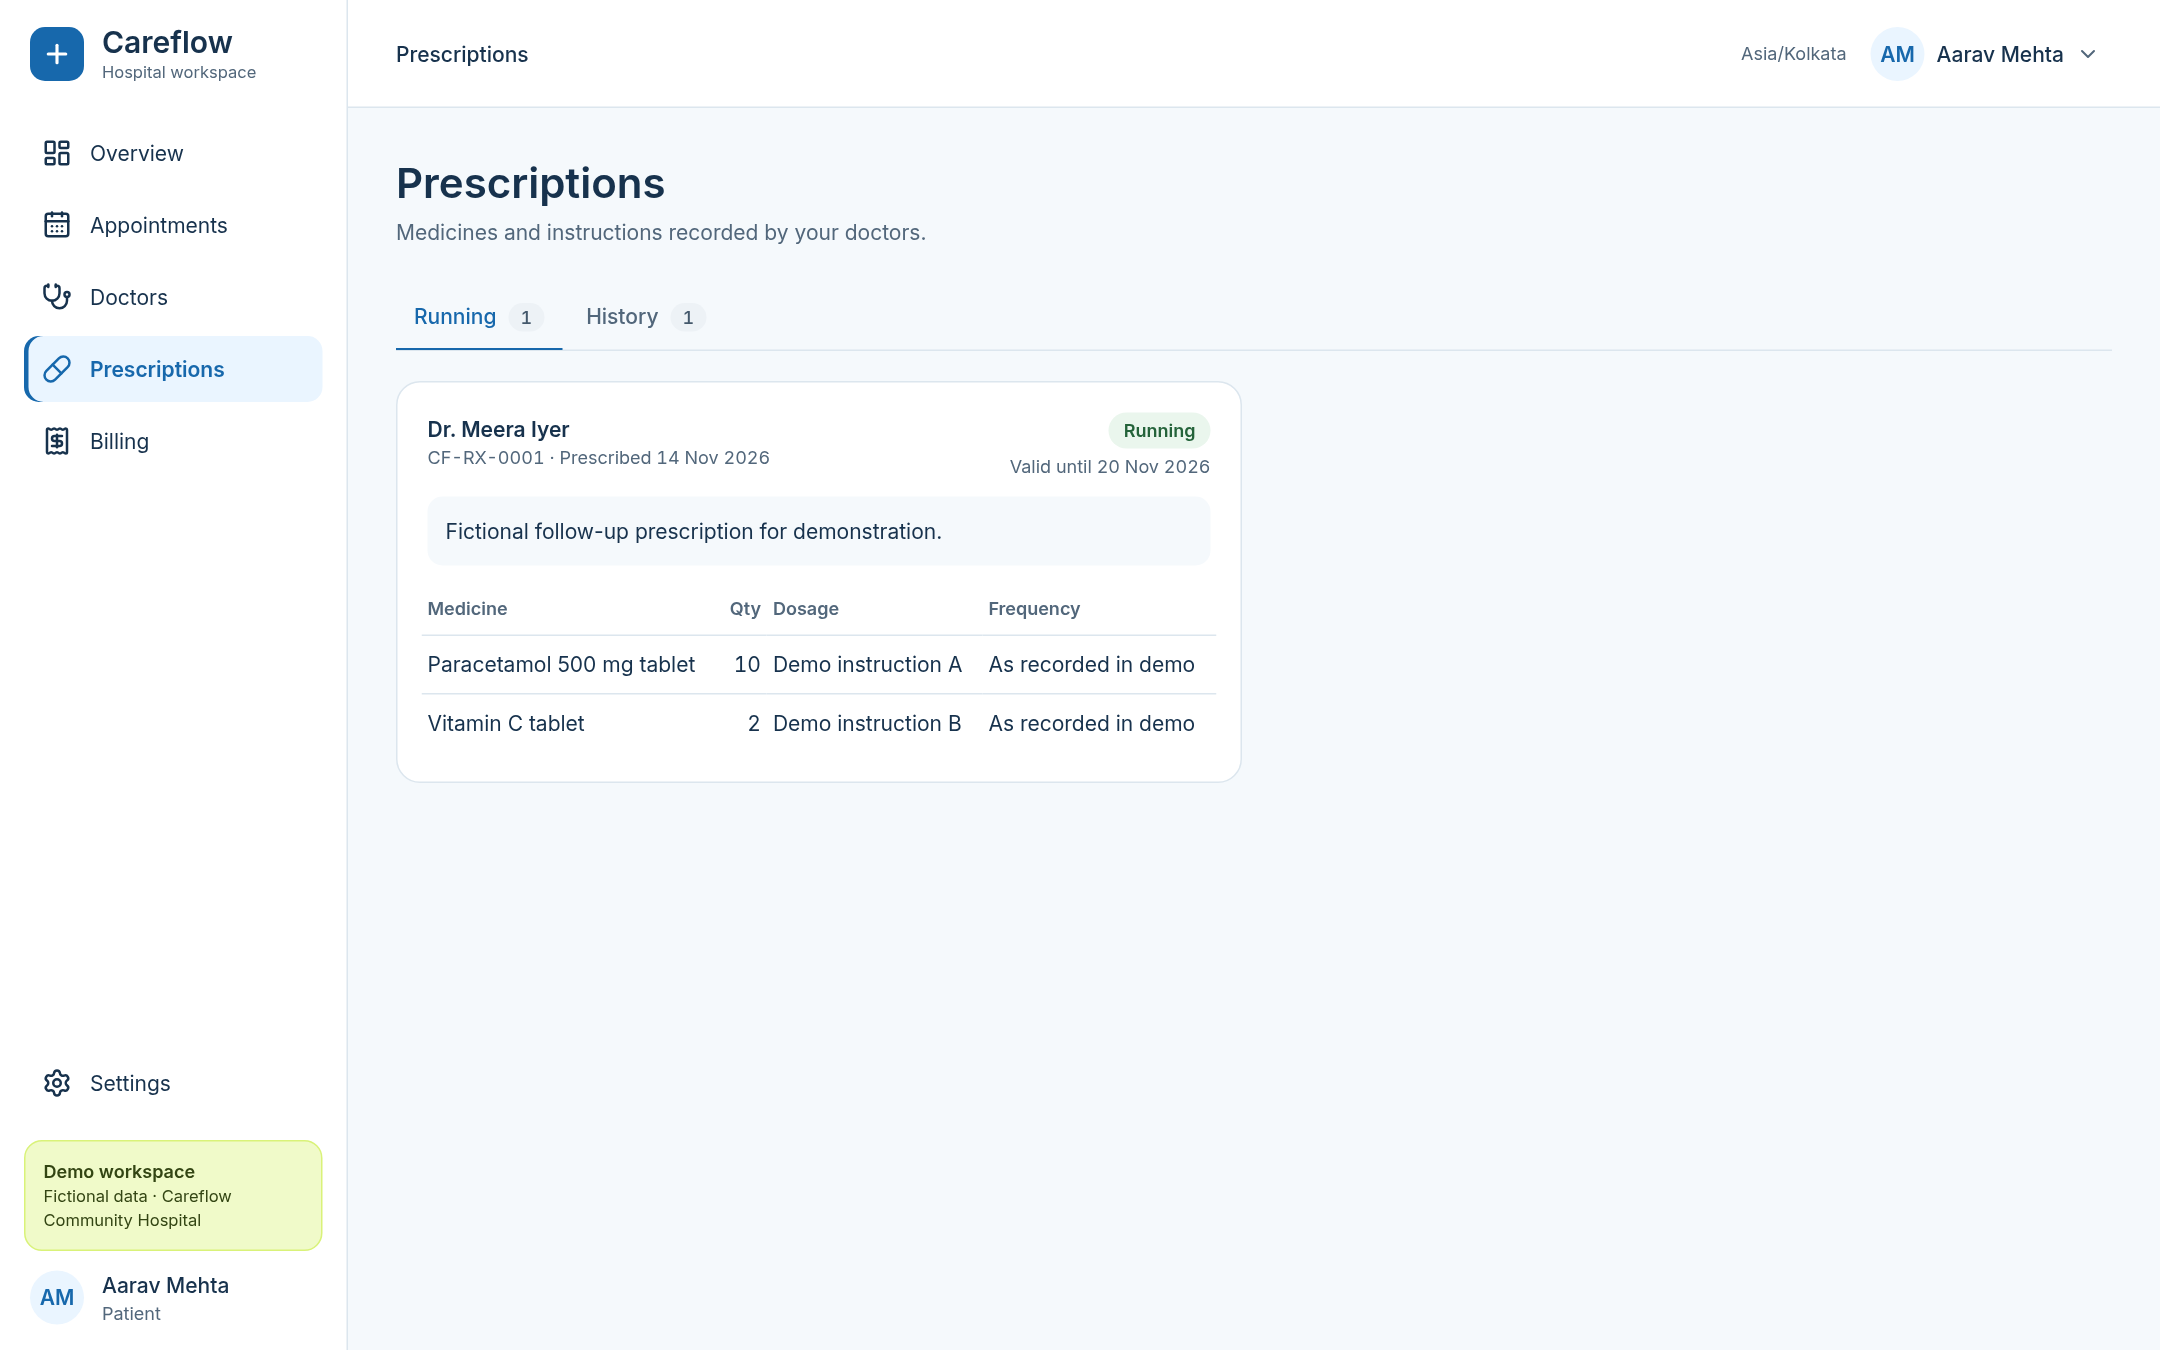
\includegraphics[width=\linewidth]{screenshots/08-prescriptions.png}\caption{Prescriptions}\end{subfigure}\hfill
\begin{subfigure}{0.49\textwidth}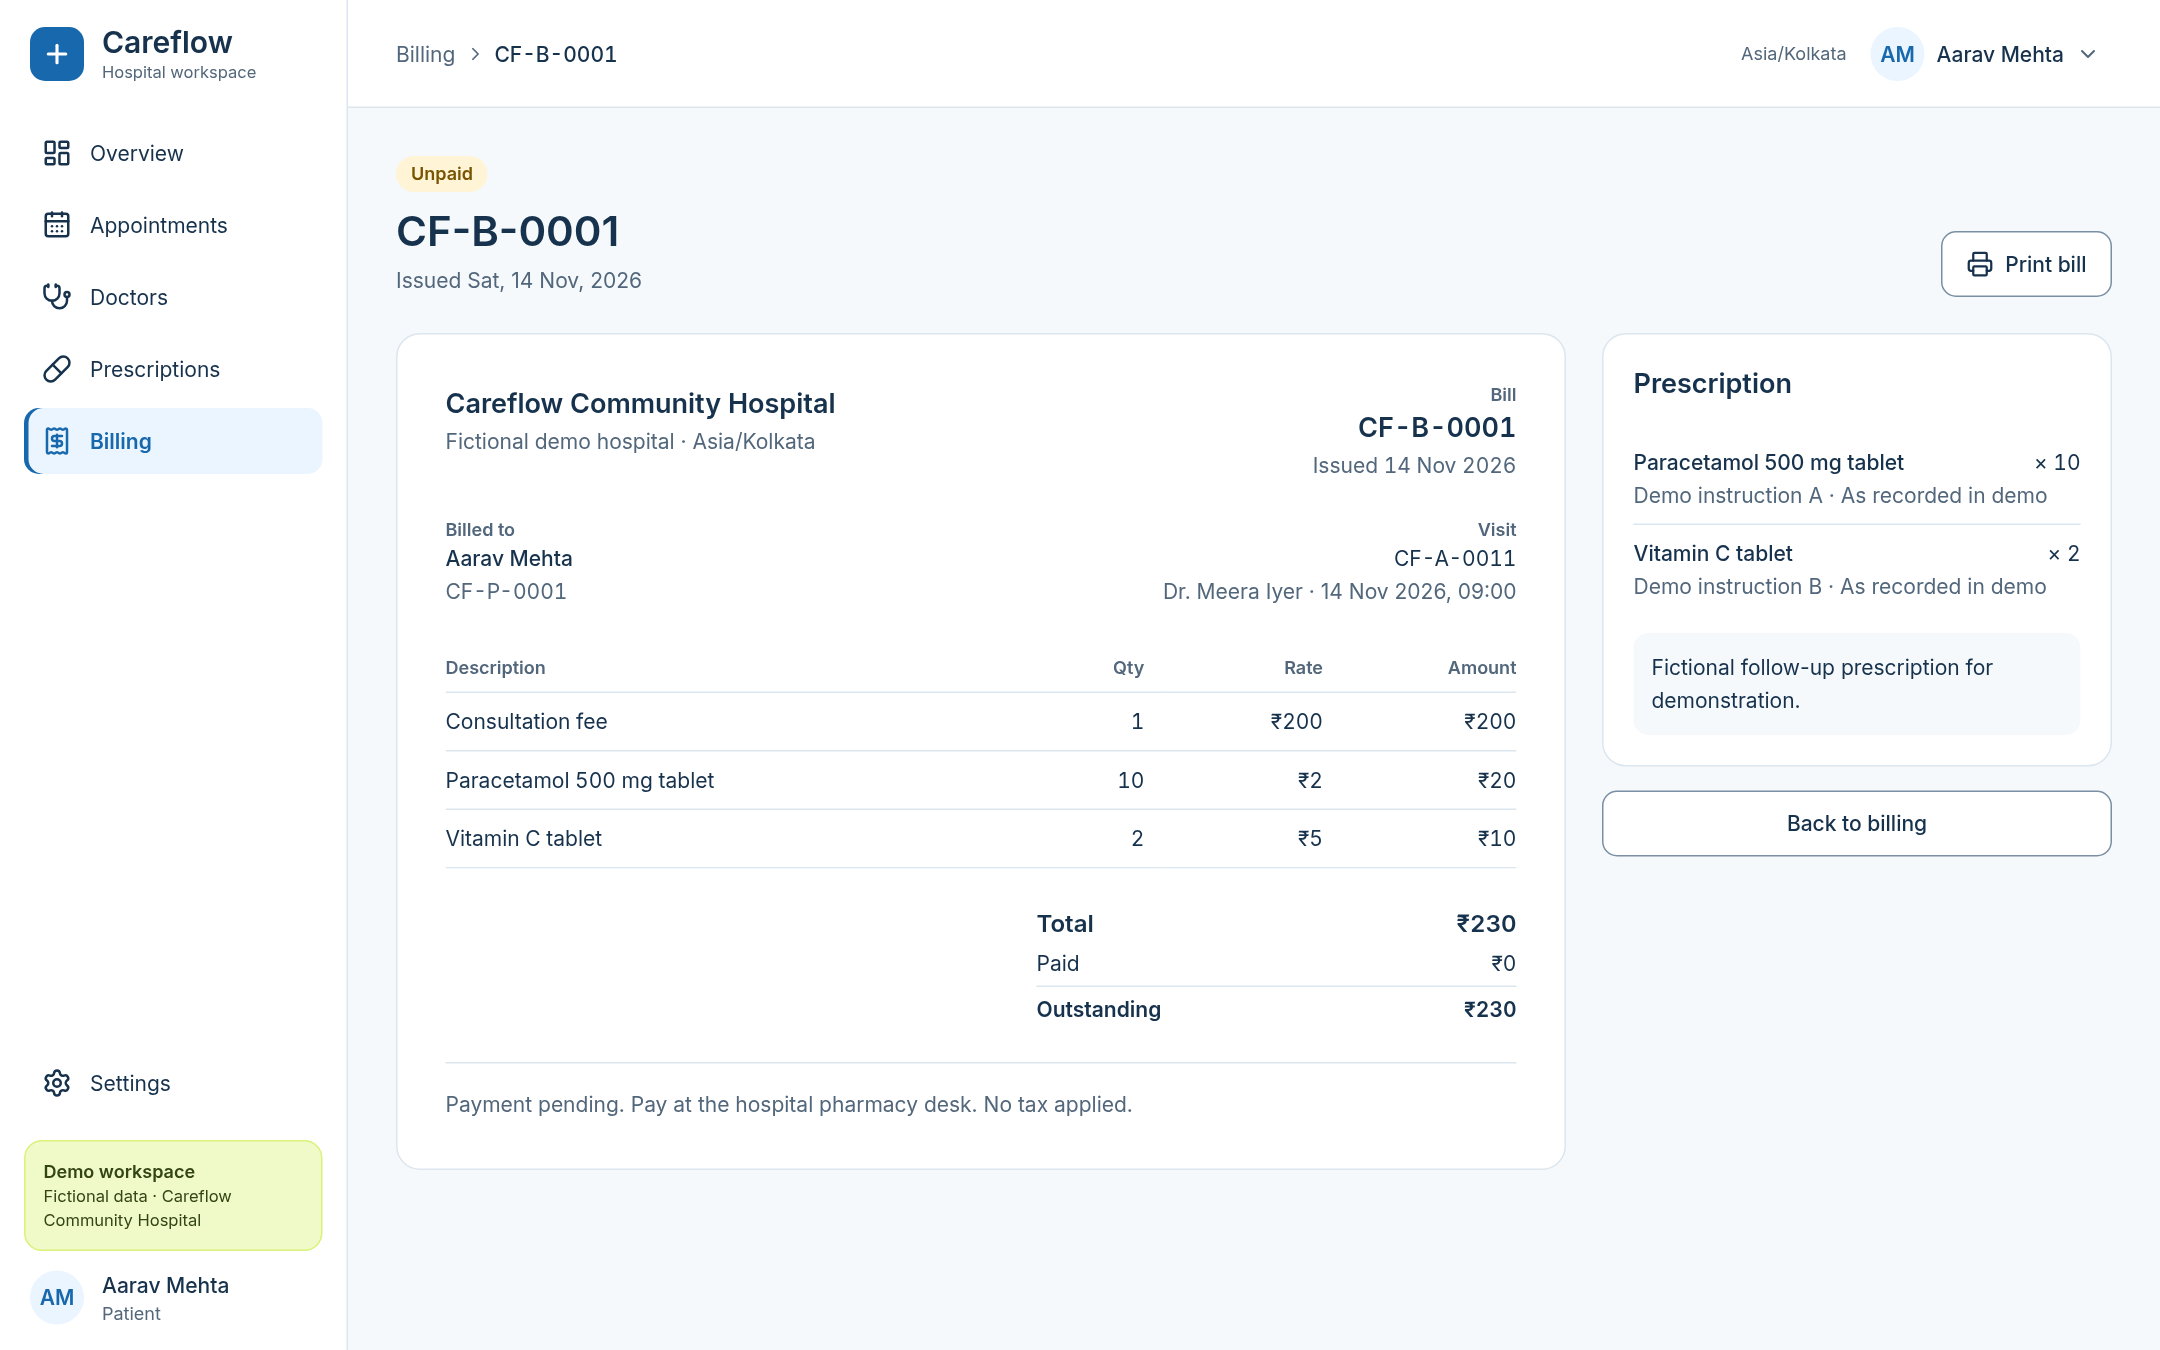
\includegraphics[width=\linewidth]{screenshots/09-patient-bill.png}\caption{Bill: consultation fee plus medicines}\end{subfigure}
\caption{Patient prescriptions and bills}
\end{figure}

\begin{figure}[H]
\centering
\begin{subfigure}{0.49\textwidth}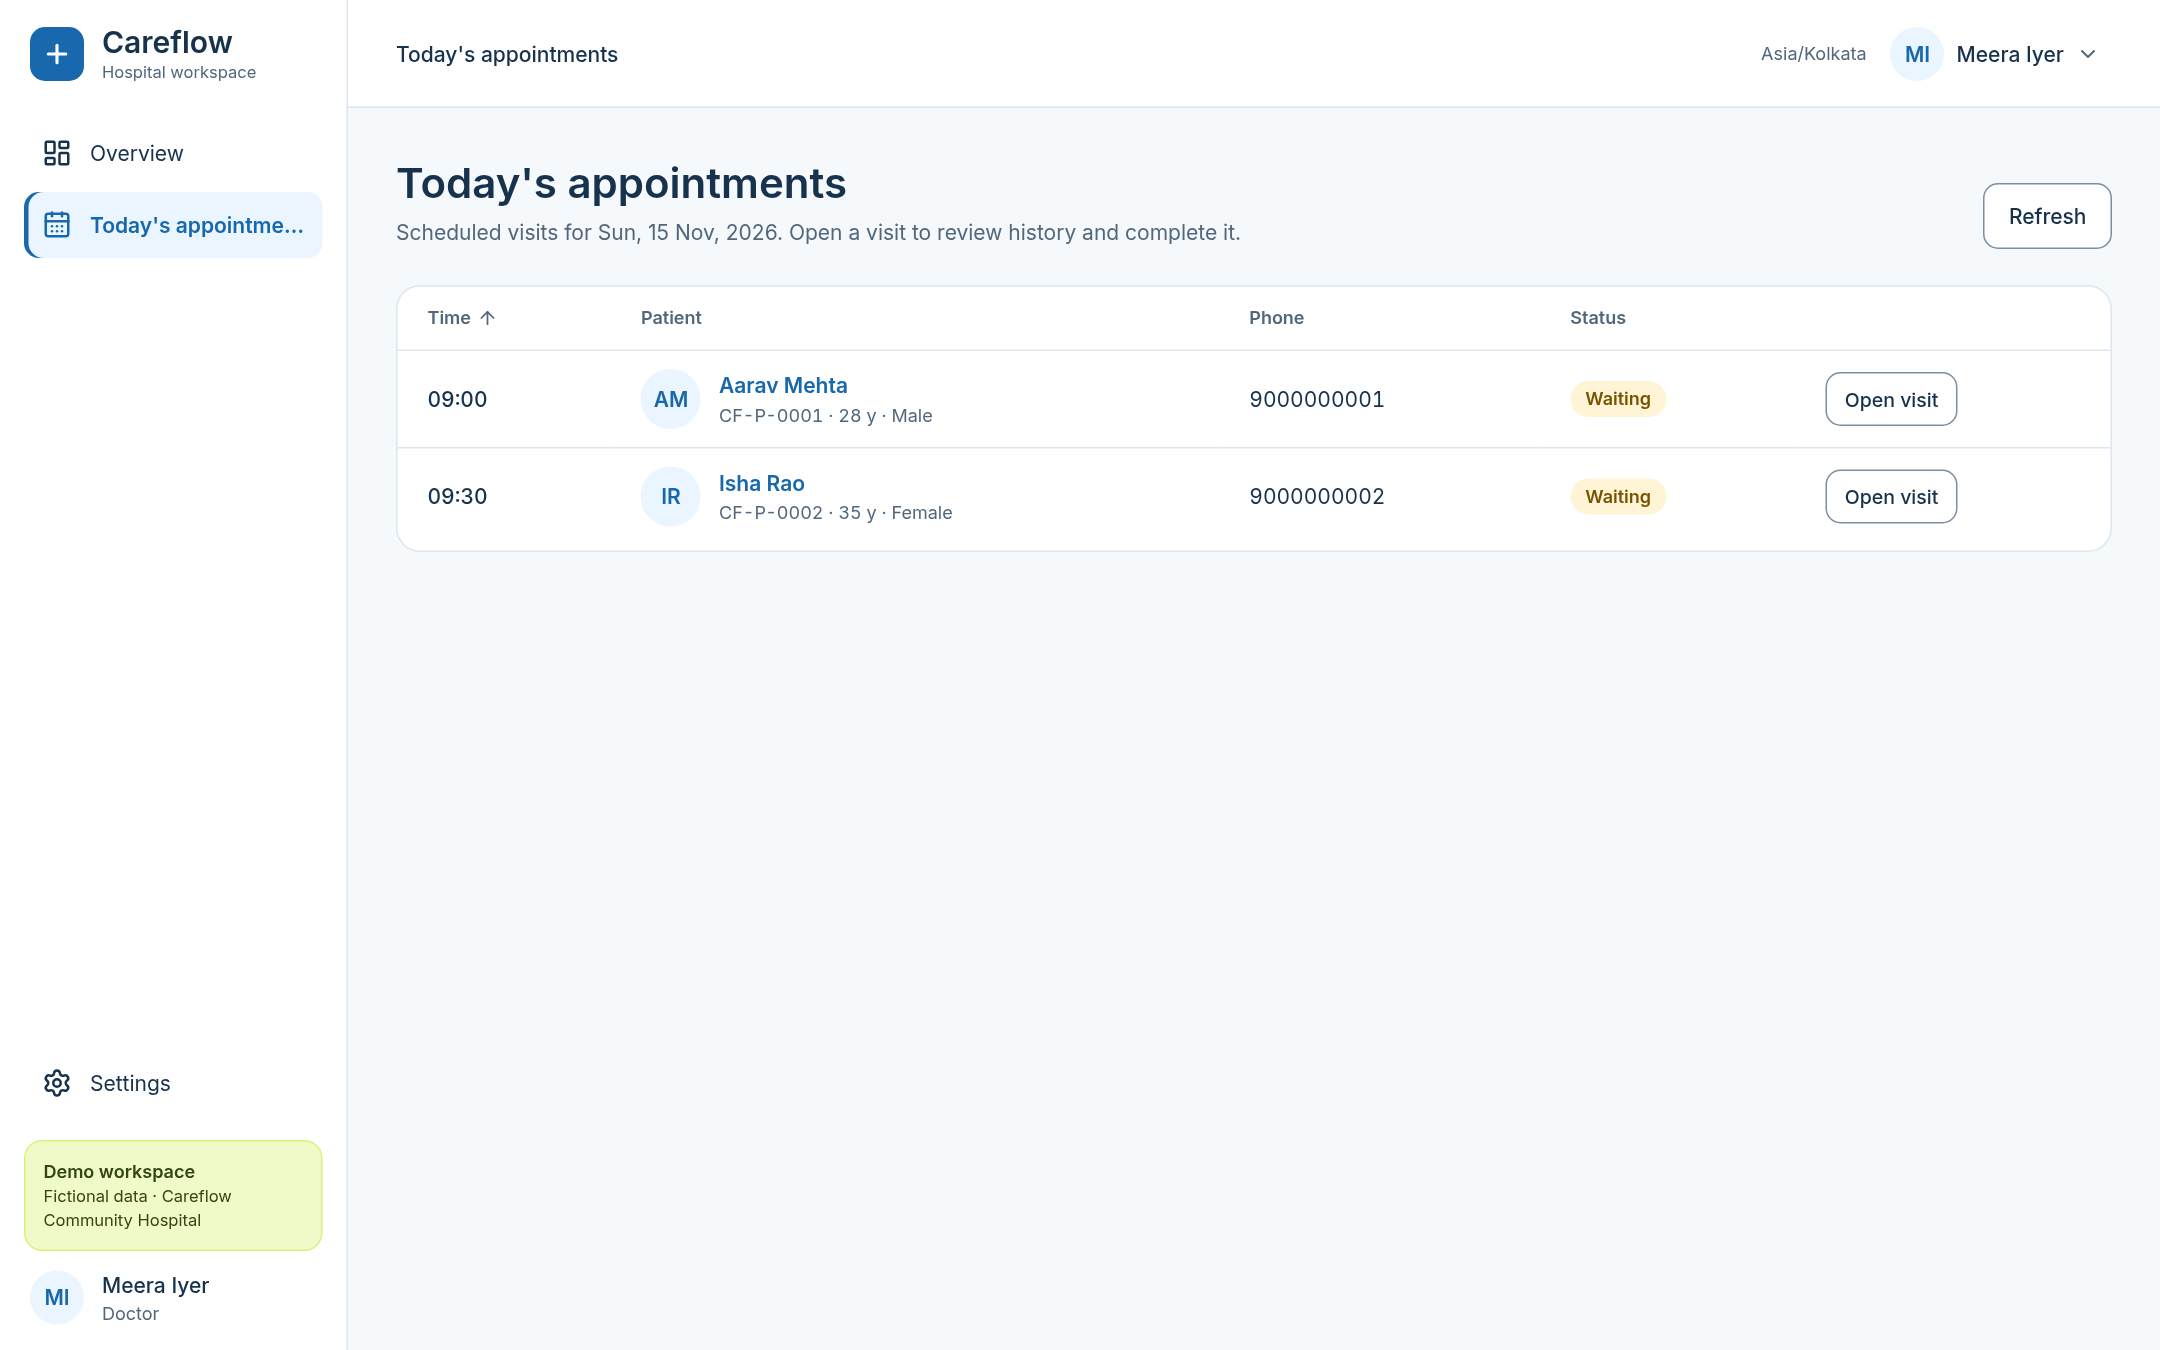
\includegraphics[width=\linewidth]{screenshots/10-doctor-queue.png}\caption{Today's queue}\end{subfigure}\hfill
\begin{subfigure}{0.49\textwidth}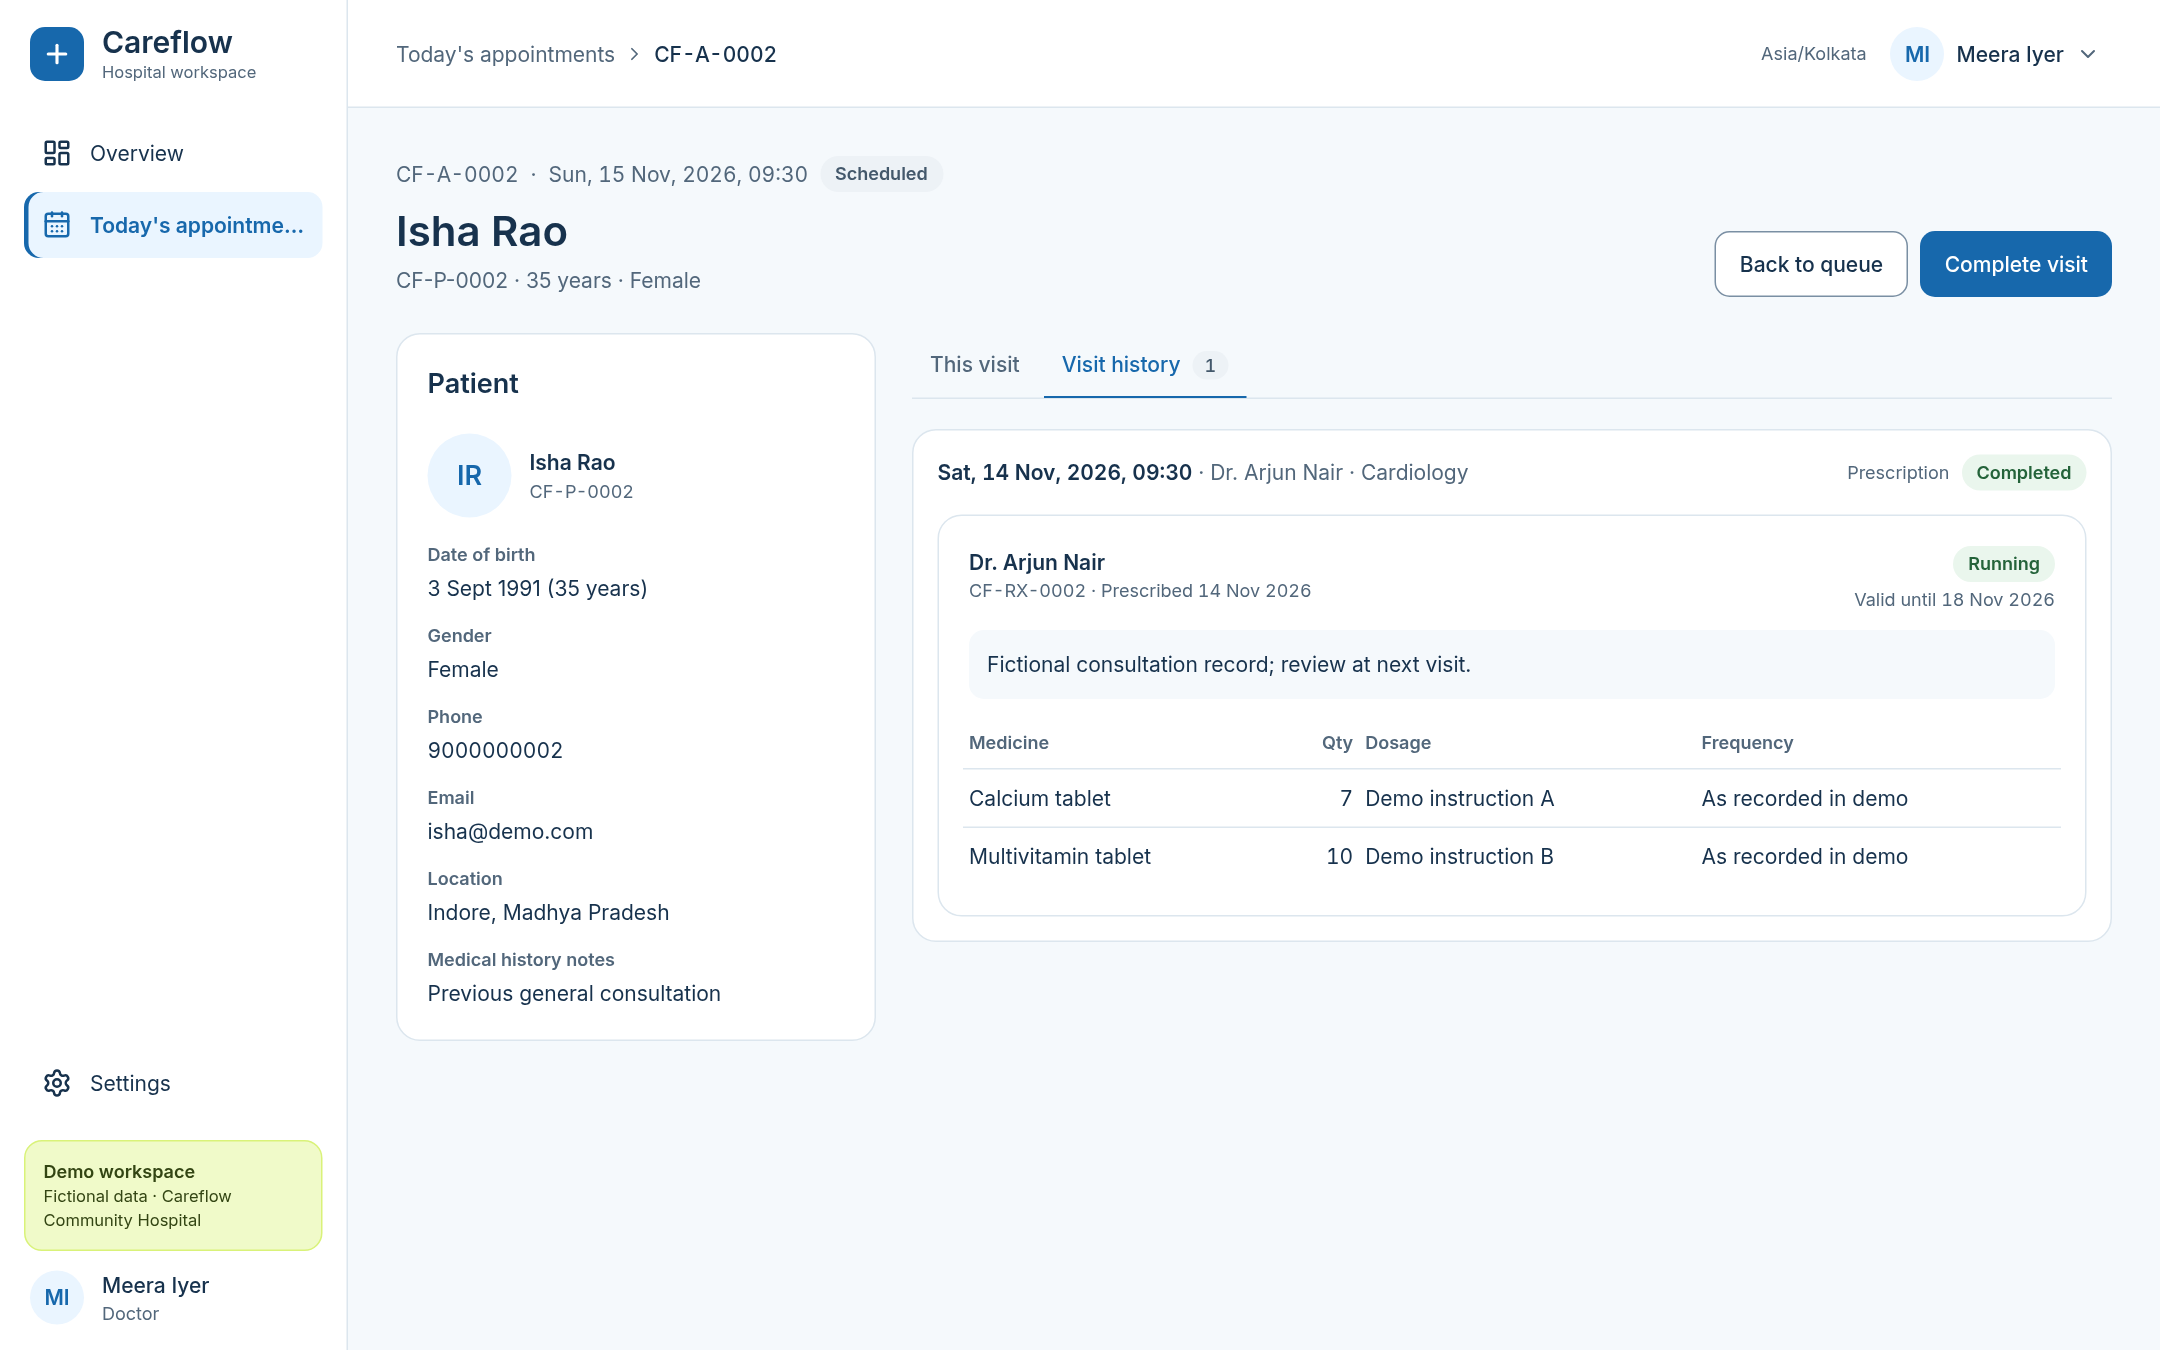
\includegraphics[width=\linewidth]{screenshots/11-doctor-visit-history.png}\caption{Patient's visit history}\end{subfigure}
\caption{Doctor screens}
\end{figure}

\begin{figure}[H]
\centering
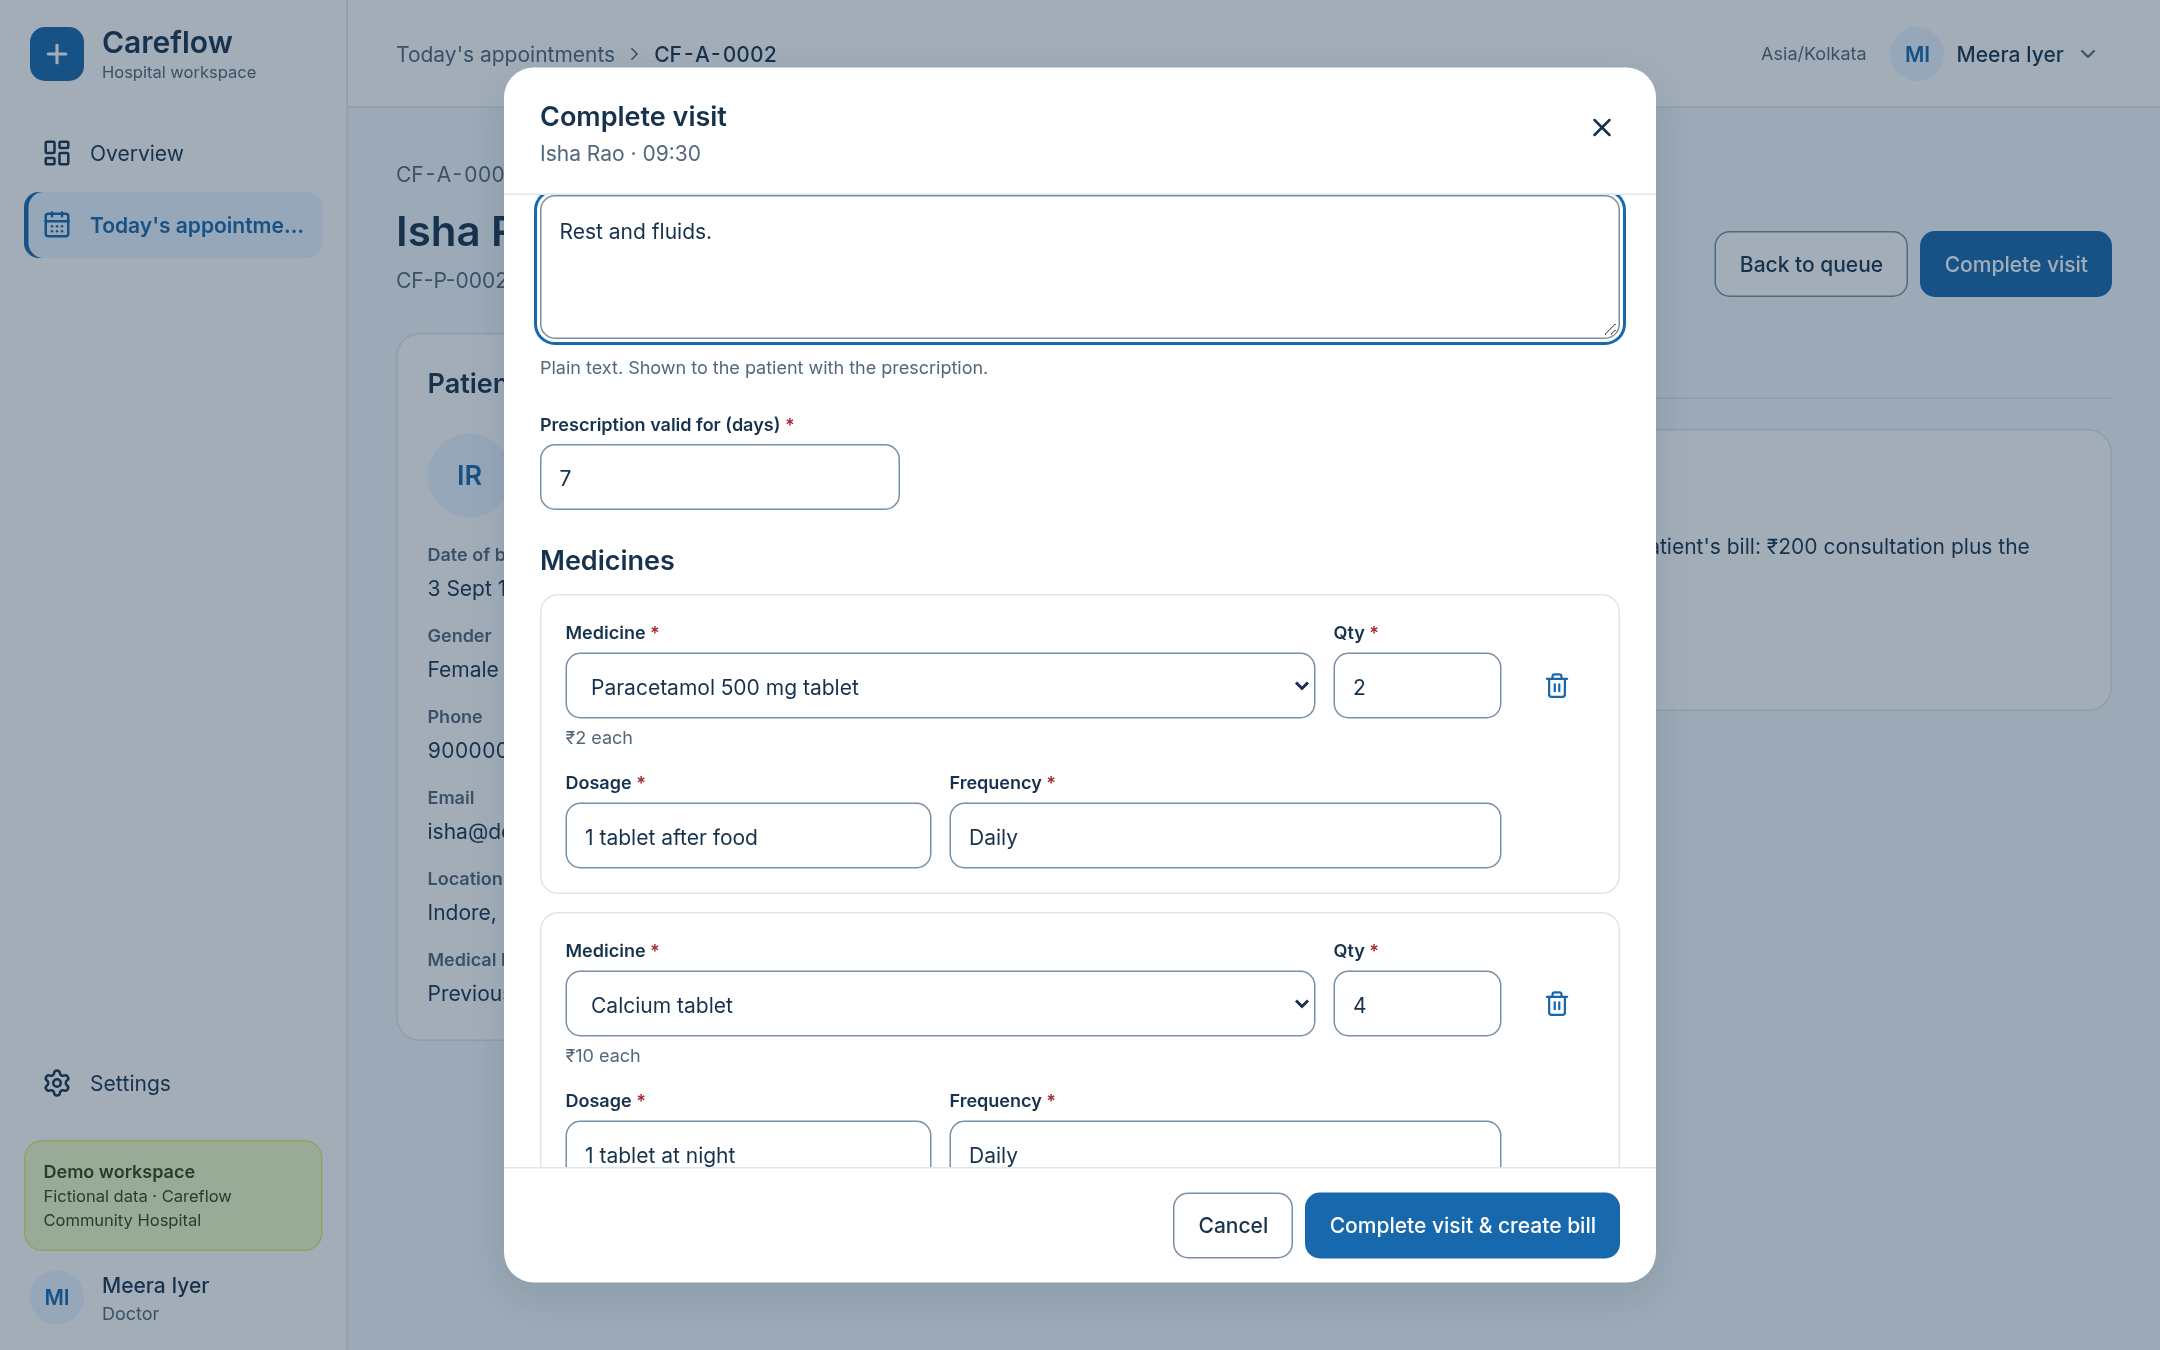
\includegraphics[width=0.9\textwidth]{screenshots/12-complete-visit.png}
\caption{Completing a visit: notes, validity and medicines. Submitting runs the complete-visit transaction}
\end{figure}

\begin{figure}[H]
\centering
\begin{subfigure}{0.49\textwidth}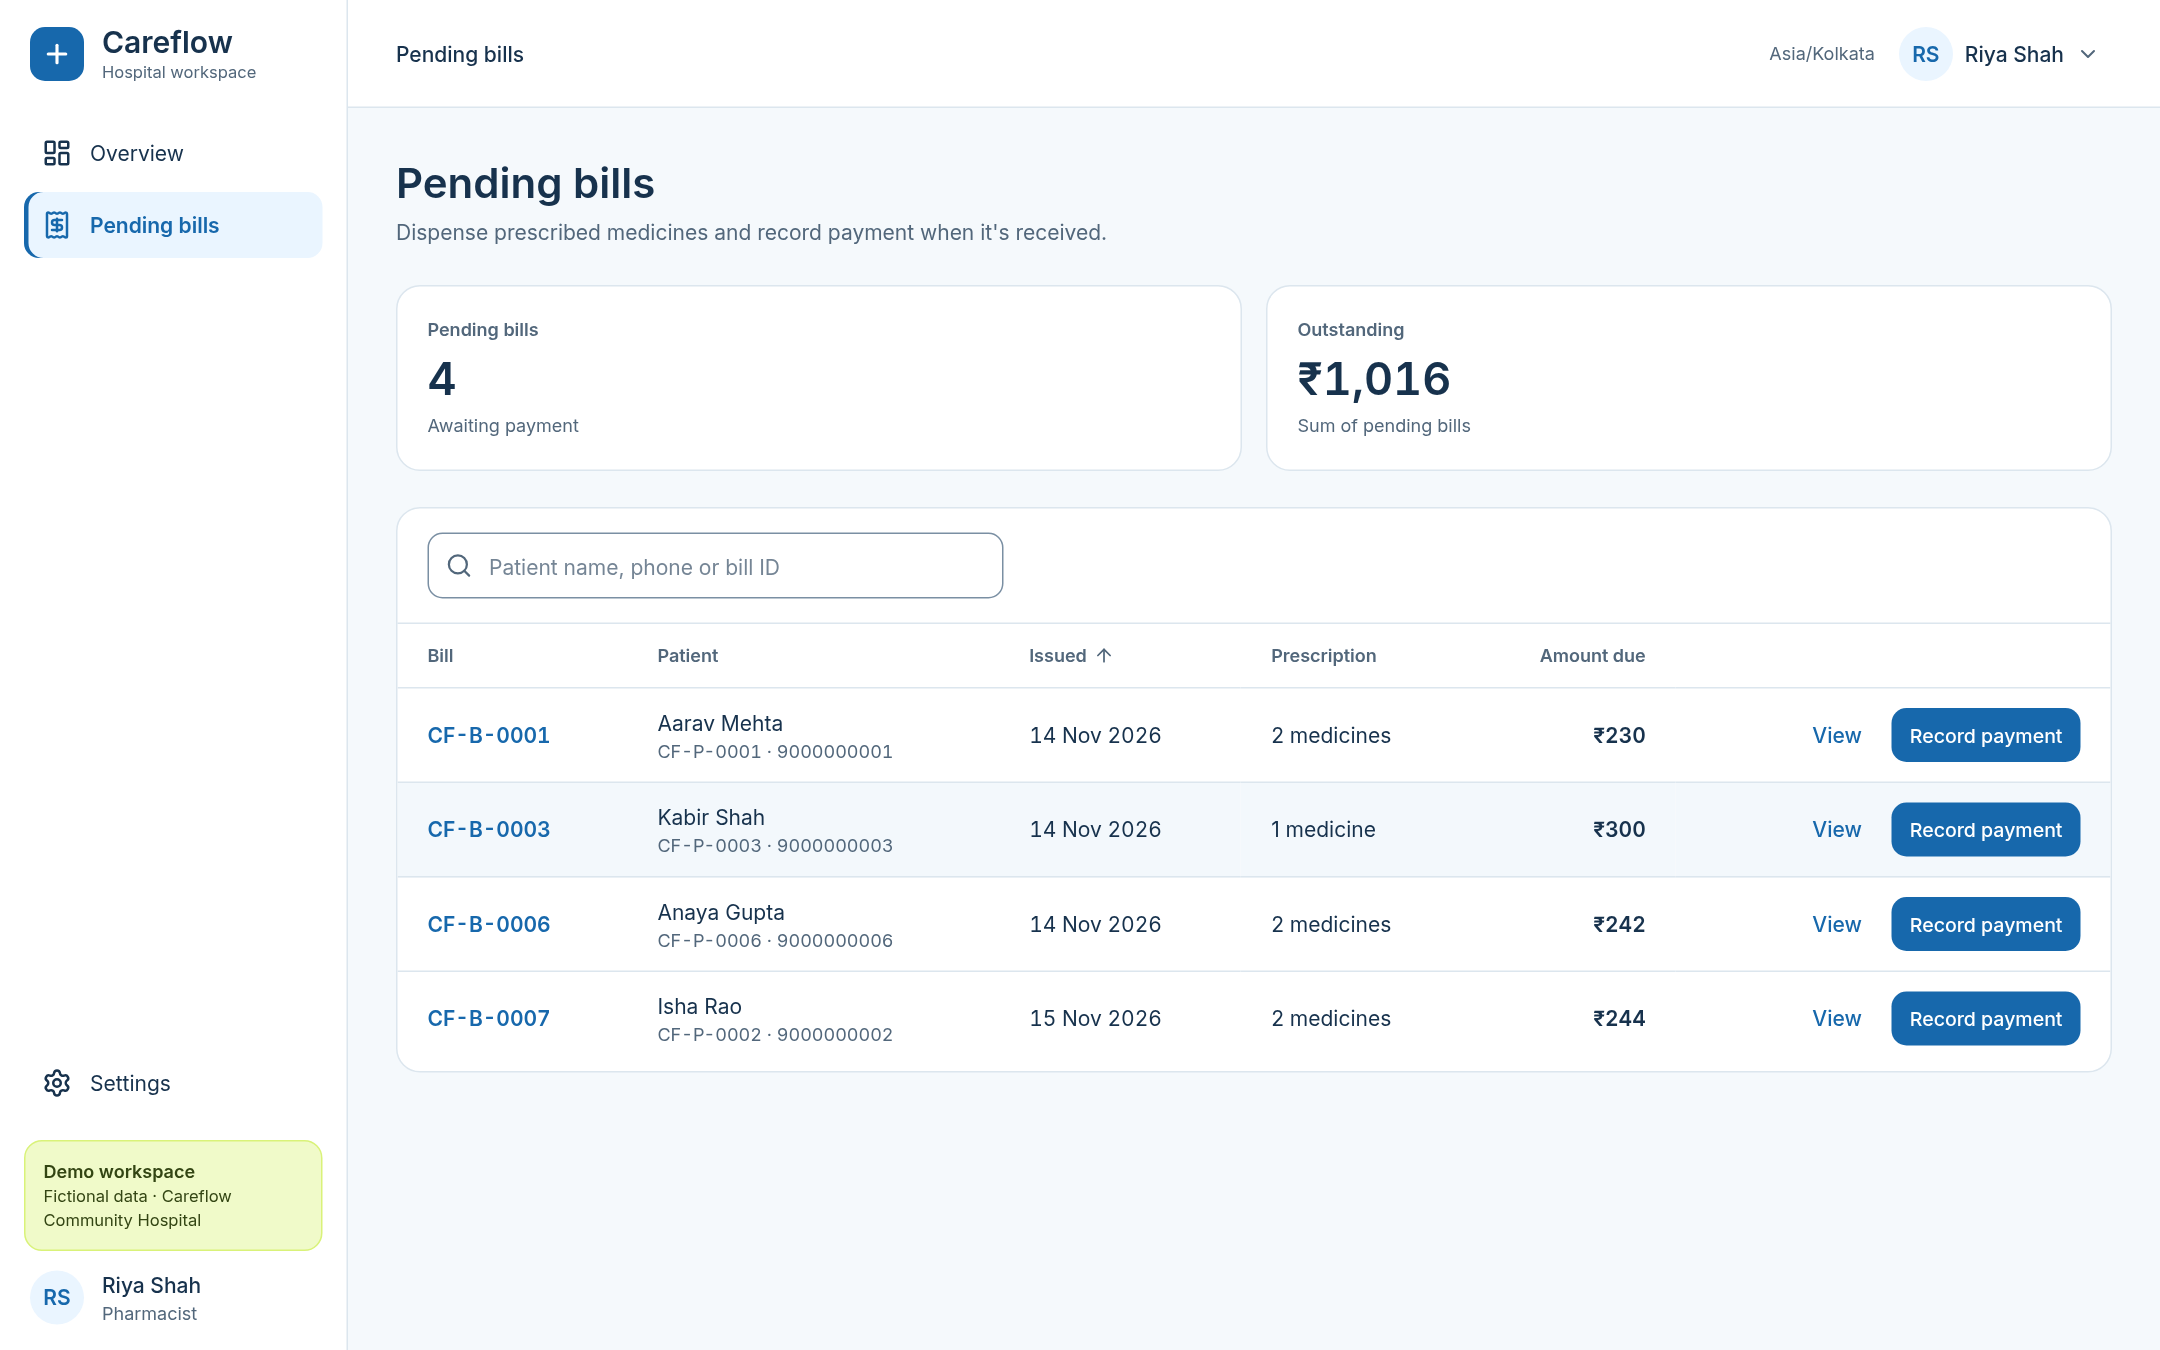
\includegraphics[width=\linewidth]{screenshots/13-pending-bills.png}\caption{Pending bills}\end{subfigure}\hfill
\begin{subfigure}{0.49\textwidth}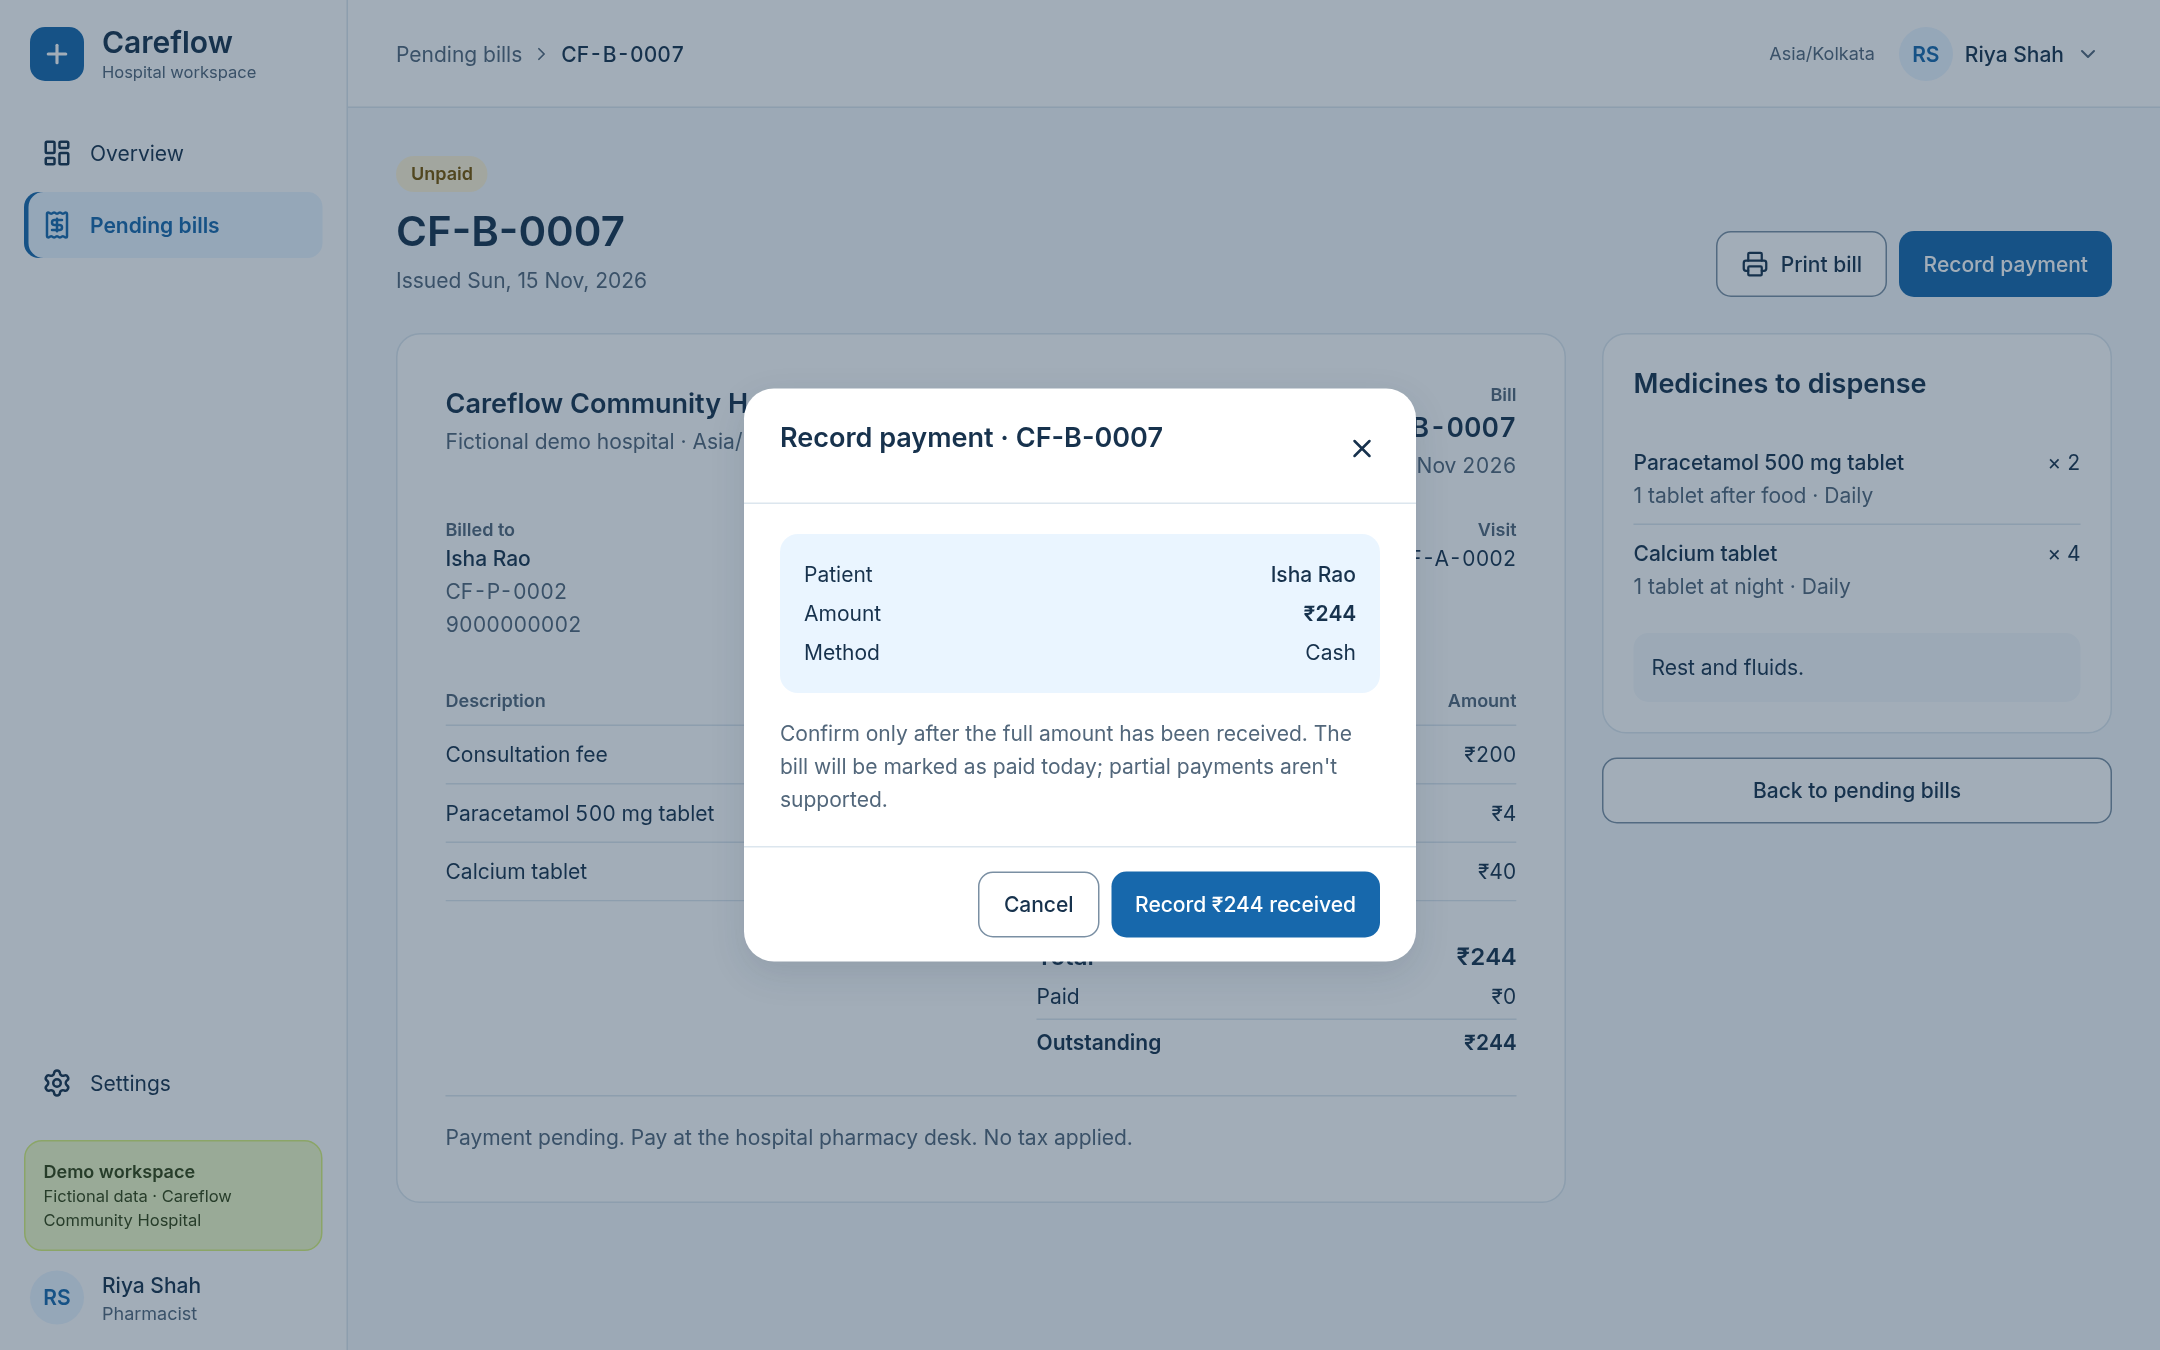
\includegraphics[width=\linewidth]{screenshots/14-record-payment.png}\caption{Recording a payment}\end{subfigure}
\caption{Pharmacist screens. The bill created in the previous figure appears here as CF-B-0007 (Rs.\,244 = 200 + 2 $\times$ 2 + 4 $\times$ 10)}
\end{figure}

\begin{figure}[H]
\centering
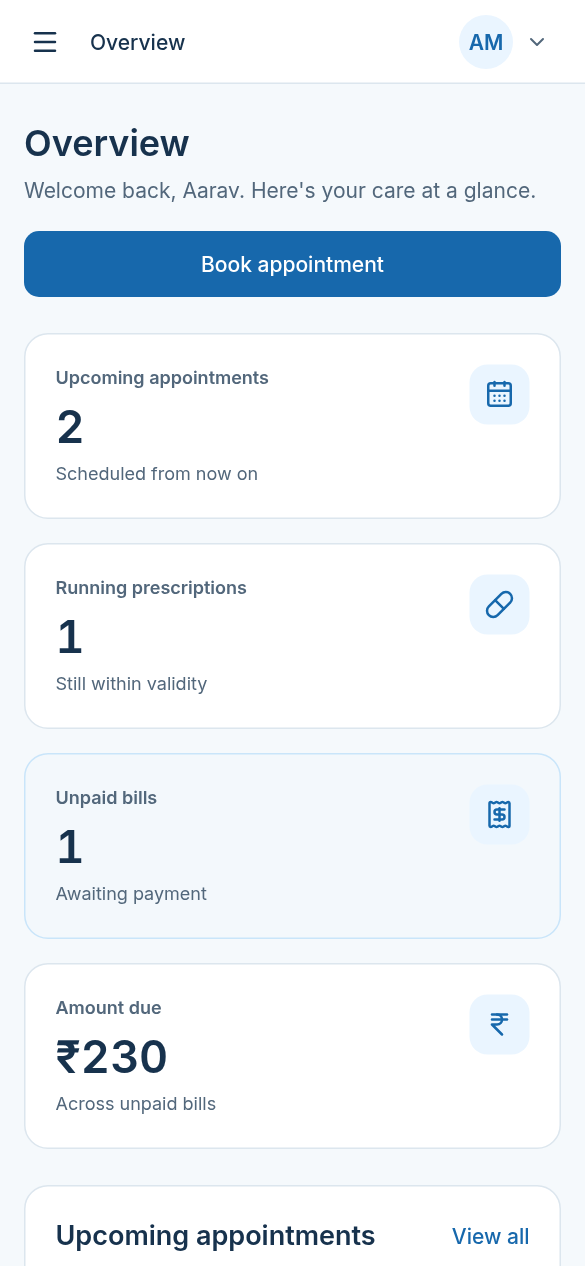
\includegraphics[width=0.32\textwidth]{screenshots/15-mobile-overview.png}
\caption{The layout adapts to phone screens}
\end{figure}

% ============================================================== 12
\section{Limitations and future work}

\begin{itemize}
  \item Technician and Admission (ward admissions) are in the ER diagram but not yet implemented as tables.
  \item The consultation fee is fixed at 200 instead of the doctor's own fee; fixing it also brings Bill to BCNF.
  \item \code{AuthAccount.Role} does not include receptionists, nurses or ward boys, so only patients, doctors and pharmacists can log in.
  \item Payments are always recorded as Cash; there is no payment gateway.
\end{itemize}

\end{document}
